\chapter{Introduction}
\label{chapter:introduction}

The main goal of this work is to design and implement a document-level text sentiment classification system with a state-of-the-art comparable performance on a practical, real-world domain of movie reviews written in Polish. For this purpose, novel strategies for regularising, pre-training and fine-tuning of recurrent neural networks known as \emph{ULMFiT} are used, combined with inductive transfer learning and subword-based tokenization methods. 

\section{Contents}

The following thesis is divided into eight chapters providing a theoretical background on sentiment classification and related machine learning problems, as well as details on the implementation of a proposed sentiment classification system.

\textbf{Chapter \ref{chapter:introduction}} introduces the main goal of this work, methods used to realise that goal and a key measurement of a proposed system's performance.

\textbf{Chapter \ref{chapter:sentiment}} defines a problem of document-level sentiment classification, discussing previous work done in the field for Polish language.

\textbf{Chapter \ref{chapter:mlbackground}} offers a theoretical background on core machine learning and deep learning concepts related to the implemented system.

\textbf{Chapter \ref{chapter:rnnnlp}} builds on the provided theoretical background by exploring key concepts behind recurrent neural networks-based natural language processing, including most notable techniques used in this field.

\textbf{Chapter \ref{chapter:projectandimplementation}} presents the reasoning behind the design of the sentiment classification system as well as details on its implementation.

\textbf{Chapter \ref{chapter:usermanual}} includes an user manual for the proposed sentiment classification system, as well as the system's platform requirements and dependencies.

\textbf{Chapter \ref{chapter:experiments}} discusses the results of experiments performed on a implemented system, validating the impact of hyperparameters on the overall accuracy of the underlying machine learning model.

\textbf{Chapter \ref{chapter:finalremarks}} summarises the accomplishments of this work, recapitulating the key insights and performance indicators of an implemented sentiment classification system.

\cleardoublepage

\chapter{Document-level sentiment classification}
\label{chapter:sentiment}

The world-wide-web revolution of early 2000s has brought new ways for people to share their opinions on a variety of subjects at a scale that has never been witnessed before in the world's history. 

Being able to \emph{mine} immense amounts of opinionated reviews, articles, blog entries or social media posts from an extensive set of sources, it is crucial to automatically process and determine their underlying sentiment in order to achieve a success in one's field. Such a problem is known as \emph{document-level sentiment classification}.

This chapter presents a background on fundamental concepts behind \emph{sentiment analysis} and \emph{document classification}, providing a reader with a perspective on the document-level sentiment classification problem for documents written in Polish language. 


\section{Sentiment analysis}

Sentiment analysis is the computational study of opinions and underlying sentiments expressed in text \cite{handbook_nlp}. The goal of sentiment analysis is to derive information from text about the entity discussed in the opinion, its assessed features (or \emph{aspects}), and the sentiment towards individual aspects of an opinion holder given in an opinion. Formally stated:

\begin{definition}
\label{def:opinion}
An opinion is a quintuple
\begin{equation}
(e, a, s, h, t),
\end{equation}
where $e$ is the target entity of an opinion, $a$ is the target aspect of the entity $e$ on which the opinion has been given, $s$ is the sentiment of the opinion on the aspect $a$ of entity $e$, $h$ is the opinion holder and $t$ is the opinion posting time \cite{liu}.
\end{definition}

A sentiment is the underlying feeling, attitude, evaluation or emotion associated with an opinion. Consumer research classifies the sentiment into two distinctive types:

\begin{enumerate}
\item \emph{Rational sentiments}, which come from rational reasoning, tangible beliefs, and utilitarian attitudes,
\item \emph{Emotional sentiments}, based on non-tangible and emotional responses to entities that are deeply connected with a person's psychological state of mind \cite{chaudhuri:2006}.
\end{enumerate}

Rational sentiments do not express any emotions and an opinion containing a rational sentiment is also referred to as an \emph{rational opinion}. For example, a sentence \textit{"This car is worth the price"} is a rational opinion. On the other hand, opinions expressing emotional sentiment, such as \textit{"I love my iPhone"} or \textit{"I am bewildered about their service personnel"} are called \emph{emotional emotions} \cite{liu}. 

Sentiments are also classified based on their positive, neutral or negative \emph{orientation} and their \emph{intensity}. A neutral orientation means that a given statement does not contain any sentiment towards the discussed entity (e.g. \textit{"This is my car"}) \cite{liu}.

Each of the sentiment types and orientations can have different strengths or intensities based on chosen words or phrases (called \emph{sentiment expressions}) and \emph{intensifiers} or \emph{diminishers} used in an opinion. For instance, using word \textit{{good}} implies lesser intensity of a statement with a positive sentiment than a word \textit{{excellent}}, and using a diminisher, such as \textit{{really}} before a word \textit{{terrible}} increases the negativity of an expression \cite{liu}. Sentiment expressions, intensifiers and diminishers are applied mainly to opinions with positive or negative sentiment orientation.

Unlike factual information, a majority of opinions is subjective. This is caused by each and every single opinion holder coming from a different background, having lived through different experiences, being concerned with different interests, ideologies and beliefs \cite{liu}. For instance, two different customers might have bought the same smartphone model, but the first customer has received a defective unit, and the other one - a properly working phone. The first customer might have a negative sentiment towards the phone (or a phone brand) if the fault is discovered, or a positive one, depending on a nature of a fault, the customers' technical knowledge and the overall satisfaction with a unit. This ambiguity poses one of the biggest challenges for the field of sentiment analysis.

\section{Natural language processing}

Natural language processing (or \emph{NLP}) is a subfield of \emph{computer science} and \emph{linguistics} that uses computer-based methods to analyse language in natural text and speech \cite{nlp_def}. The goal of NLP is to develop techniques allowing for near-human-level accuracy in tasks such as sentiment analysis, \emph{natural language understanding}, \emph{speech recognition} or \emph{natural language generation}.

Natural Language Processing has relied on the developments in the field of \emph{artificial intelligence} (\emph{AI}), evolving from \emph{symbolic} approaches (based on manually defined sets of rules) to more modern, statistics-based methods for problem-solving \cite{handbook_nlp}.

Many recent breakthroughs in NLP brought by \emph{deep learning} have made it possible for automatic language translators and voice assistants, for instance, to become ubiquitous and indispensable parts of our everyday life.

\subsection{Document definition}

In NLP, \emph{document} is an entity containing a distinct text. For instance, a single document might contain the entire contents of a single book, as well as an individual article.

In this work, a term document is used interchangeably with \emph{text document} to emphasise the nature of document's contents.

\subsection{Text classification}

\emph{Text classification} is a fundamental natural language processing task of assigning a label $l$ for an input text document $t$ from a defined set of labels $C$ known as \emph{classes} based on predefined criteria. It has broad applications in the fields of sentiment analysis, topic labelling and spam detection, among others \cite{wiki:doc_classification}.

For example, having a set of labels $C = \{\mathrm{e-mail}, \mathrm{spam}\}$ and input e-mail subjects $t_1 =$ "WIN LOTTERY, REWARD!" and $t_2 = $ "Report from Research, May 2019" the goal of a text classification of e-mail subject texts is to produce pairs $(t_1, l_1)$ and $(t_2, l_2)$, where $l_1 = $ "spam" and $l_2 = $ "e-mail".

\section{Document-level sentiment classification}
\label{document-level-sentiment-classification}

Document-level sentiment classification, also referred to as or \emph{document sentiment analysis} or \emph{document sentiment classification}, is a task of classifying an \emph{opinionated document} as expressing a positive, neutral or negative opinion (or sentiment) \cite{handbook_nlp}.

It is assumed in document sentiment analysis that the opinionated text document expresses opinions on a single entity $e$ and contains opinions from a single opinion holder $h$ \cite{liu}. Thus, in order for a document to be properly classified using document-level sentiment classification, it should not contain opinions expressed on different entities, or by multiple authors on a single entity.

Considering an example opinionated document containing a review of a book from Amazon.com:

\begin{remark}{}
\label{ex:1}
"Thrilling read. If you're having trouble sleeping this is perfect for reading just before bed. If you're wide awake and want to learn how to write and publish a scientific paper, it works for that too. I'm a grad student and this book was recommended to me by a prof from my undergrad university and it was worth every penny. It helped me get better at analysing the quality of writing by others \cite{amazon:review}."
\end{remark}

an accurate document sentiment classification determines the example document to be positive in terms of the opinion holder's $h$ sentiment towards a book entity $e$.

Document-level sentiment classification task treats sentiment classification as a traditional text classification problem with sentiment orientations as classes \cite{liu}. As such, applications of a supervised learning-based solutions are used as a basis for modern document sentiment analysis systems.

\section{From symbolic to neural networks-based approaches to NLP and document sentiment analysis}

Classical approaches to NLP have their roots in \emph{symbolic artificial intelligence}, based on the knowledge of the field of linguistics and involving meticulous analysis of texts using many predefined sets of rules \cite{handbook_nlp}. 

Modern natural language processing is, contrary to symbolic approaches, heavily based on the latest developments in the area of \emph{deep learning}. Combining classical methods, such as word \emph{tokenization}, with the \emph{deep neural networks}' ability of learning accurate representations of data has allowed for state of the art results in a variety of NLP tasks to be achieved, including text classification, sentiment analysis and machine translation \cite{ulmfit,languagemodels:vstranslation,goodfellow,pan:sentimentanalysis,zhou:sentimentcnn}.

After an introduction of core machine learning and deep learning concepts in chapter \ref{chapter:mlbackground}, \emph{recurrent neural networks-based} approaches to natural language processing and, specifically, the problem of document sentiment classification are discussed in chapter \ref{chapter:rnnnlp} of this work.

\section{Polish document sentiment classification}
\label{sentiment:polish}

Polish language belongs to a family of highly inflected languages, in which a form or ending of a word depends on it's use in a sentence, reflecting a grammatical tense, case, voice, aspect, person, number, gender, mood, and others \cite{wiki:inflection}. Combining a complex grammar with an extensive set of exceptions, Polish language has been perceived as difficult for automated natural language processing \cite{polish:difficult,polishdiff,polishdiff_grammar}.


This section introduces a neural network-based approach to the problem of the Polish document-level sentiment classification, as well as provides an outlook on the previous work done on this subject for Polish opinions.

\subsection{This work}

As the aim of this work is to produce a document-level text sentiment classification system with a state-of-the-art comparable performance, the resulting system is based upon \emph{deep recurrent neural networks}.

The ULMFiT method has been chosen as a foundation of the system, used to produce a final \emph{target classifier} model. Based on promising results from previous works \cite{czaplakardas:ulmfit,poleval2019}, a \emph{sentencepiece}-based tokenizaton method is used on two separate, real-world corpora - \emph{plwiki} and \emph{Filmweb+}, specifically prepared for use in this work.

Compared to previous work (see \ref{previouswork}), our document sentiment classification system is trained on relatively small labelled dataset, Filmweb+, consisting of just 3085 positive and 3085 negative example documents, with an average length of 514 words per document.

Also, the results of this work can be reproduced using commercially available hardware, with the process of pre-training and fine-tuning language models and training target classifier taking less than 10 hours of computing time on \lstinline{Nvidia GeForce 2080Ti} graphics card.

The motivation between the design and implementation choices made is provided in chapter \ref{chapter:projectandimplementation} of this work, and a theoretical background - in chapter \ref{chapter:mlbackground} and \ref{chapter:rnnnlp}.

\subsection{Previous work}
\label{previouswork}

Previous work on the Polish text document sentiment classification has been based on classical NLP approaches \cite{buczynski:shallowclassicalnlp,wojcik:comparisonclassicnlp}, \emph{Bayesian} \cite{wiki:bayesian, chlasta:sentimenttwitter,polish:sentimentbayesian} and \emph{support-vector machines}-based \cite{wiki:svms,polish:sentimentsvms} classification methods, as well as deep neural networks \cite{czaplakardas:ulmfit,korzeniowski:poleval,wawer:polishsentimentshorttexts,poleval2019}, with the latter producing state-of-the-art results for a Polish language at the time of writing this thesis.

However, a vast majority of the work on document-level sentiment classification has been performed on \emph{corpora} consisting of relatively short texts, such as posts from Twitter \cite{poleval2019,korzeniowski:poleval,chlasta:sentimenttwitter}, short user rating comments from Filmweb \cite{wawer:polishsentimentshorttexts} and Opineo store and product reviews \cite{polish:sentimentsvms}. In fact, no recent work on Polish document sentiment analysis that involved use of a dataset consisting of long (over 1000 characters on average), real-world documents.

Some of the neural networks-based approaches to document-level sentiment classification have leveraged the \emph{pre-training} and \emph{fine-tuning} of \emph{language models} as well as \emph{inductive transfer learning} \cite{czaplakardas:ulmfit,poleval2019,korzeniowski:poleval,wawer:polishsentimentshorttexts}, using methods known \emph{Universal Language Model Fine-Tuning} (or \emph{ULMFiT}) \cite{ulmfit} and \emph{Bidirectional Encoder Representations from Transformers} (or \emph{BERT}) \cite{bert}. Both of these methods have produced satisfactory results.













\chapter{Background on machine learning}
\label{chapter:mlbackground}

The following chapter introduces the core problems of machine learning and deep learning involved with a recurrent neural networks-based natural language processing systems used to perform document-level sentiment classification. 

It defines core concepts, such as \emph{transfer learning}, \emph{regularisation}, \emph{backpropagation} and \emph{recurrent neural networks} referred to in the latter parts of this work.

\section{Machine learning}

\emph{Machine learning} (or \emph{ML}) is a subfield of \emph{artificial intelligence} that gives computers the ability to learn without being explicitly programmed \cite{samuel_def_ml}. 

\begin{figure}[]
\centering
\includegraphics[scale=0.35]{figures/ai_venn.png}
\caption{A diagram illustrating the relationships between the fields of artificial intelligence, machine learning, representation learning and deep learning \cite{goodfellow}.}
\label{ai:diagram}
\end{figure}

A formal definition of \textit{learning} is provided by Tom Mitchell \cite{mitchell_def_learn}:

\theoremstyle{definition}
\begin{definition}{}
\label{ml:def}
A computer program is said to learn from experience $E$ with respect to some class of tasks $T$ and performance measure $P$, if its performance at tasks in $T$, as measured by $P$, improves with experience $E$.
\end{definition}

To put a definition \ref{ml:def} in layman's terms, a computer program learns when it is able to interpret new data (experiences $E$) in such a way, that it is able to solve a given problem (task $T$) with a better outcome (as measured by $P$).

Machine learning-based classification systems, for instance, learn how to accurately label a provided input by being presented with a set of example inputs for each category called the \emph{training set}. For such systems:
\begin{enumerate}
\item The task $T$ is to classify an input based on its distinctive features,
\item The experience $E$, from which a computer program learns, is a \emph{sample} from a training set,
\item The performance measure $P$ can be defined in numerous ways deemed appropriate; commonly, ratio of correctly classified inputs - a metric called \textit{accuracy} - is used.
\end{enumerate}

Sentiment classification system is an example of such a system, for which the task $T$ is to classify an opinionated document based on its contents and an experience $E$ is an individual, already labelled document. A $P$ can be measured by an accuracy, \emph{precision} or \emph{F1 score} metrics, among others. 

% TODO: ADD SOMETHING MORE ON METRICS

A core part of the machine learning system is called a machine learning \emph{model}, which is an entity that has obtained the knowledge from all the experiences $E_i \in \{E_1, \dots, E_n\}$ belonging to a training set. The process of presenting a machine learning system with new examples from a training set is called \emph{training}.

Machine learning is a broad field in its own, with many subfields, most notable of which include \emph{representation learning} and \emph{deep learning}. A relation between artificial intelligence, machine learning and its subfields is shown in figure \ref{ai:diagram}.

\subsection{Types of machine learning systems}

Machine learning systems are classified based on the human input needed during the training process into:

\begin{enumerate}
\item \emph{Supervised learning} systems, which learn how to interpret new data given some input data with associated, desired outputs (or \emph{labels}),
\item \emph{Semi-supervised learning} systems, which learn from input data for which only some labels are available,
\item \emph{Unsupervised learning} systems, which learn the correlations between given \textit{unlabelled} input data.
\end{enumerate}

% add reinforcement learning
% up up up

\subsection{Inductive and transductive learning}

\emph{Transduction}, in the context of statistical learning, refers to predicting specific results of drawing from a given set of examples. A classical example of a transductive algorithm is the \emph{K-Nearest Neighbours} algorithm, which uses the training data directly to make a prediction.

% Read more on transduction in NLP, whether it's used in ulmfit or not

Contrary to transduction, \emph{induction} in machine learning is a process of deducing general rules from observed training cases.

\subsection{Representation learning}

The performance of machine learning systems depends heavily on a \emph{representation of data} used \cite{bengio2012representation}.

An example ML system based on a \emph{logistic regression} algorithm \cite{logreg_caesarian} used to recommend a cesarean delivery produces its output based on an input vector of features, representing neonatal birth weight or gestational age at birth, among others. Such a system requires its operator to manually \emph{pre-process} input data not only for the purposes of training, but also - in this case - in order to produce a valid classification. 

\begin{figure}[]
\centering
\includegraphics[scale=0.3]{figures/representation.png}
\caption{Using a different representation of data may result in a much simpler solution for a target machine learning task. In this example, a change of coordinate system from Cartesian to polar allows to perform a classification of objects belonging to class of dots and triangles by separating them with just a single line \cite{goodfellow}.}
\label{representation:cartesianvpolar}
\end{figure}

In general, much of the actual effort involved in deploying a machine learning algorithm has involved the design process of task-oriented pre-processing pipelines and data transformations, resulting in a representation of data that allows for accurate outputs, as illustrated in figure \ref{representation:cartesianvpolar} \cite{bengio2012representation}.

However, many problems cannot be solved through a manual engineering of data representations. Automated face detection, for example, was an unsolvable problem until as recently as the year 2001 \cite{face2001, introductiontoml}, when an integral image representation was first proposed.

This difficulty has lead to an emergence of \emph{representation learning}, a set of machine learning techniques which allow a system to automatically discover the representations needed for a given task and replace a tedious, aforementioned process called \emph{feature engineering} \cite{wiki:representation_learning}.

Current proliferation of object detection, speech recognition or NLP systems \cite{bengio2012representation}, among others, is attributed to the emergence of effective representation learning methods, such as \emph{deep learning}.

\subsection{Transfer learning}

\emph{Transfer learning} refers to a machine learning algorithm's ability of exploiting commonalities between given learning tasks \cite{bengio2012representation} through an use of knowledge obtained in one learning task in order to improve a system's performance in another task.

%A more mathematical transfer learning definition: http://ict.usc.edu/pubs/Inductive%20Transfer%20Learning%20for%20Handling%20Individual%20Differences%20in%20Affective%20Computing.pdf

\begin{figure}[]
\centering
\includegraphics[scale=0.15]{figures/transfer.png}
\caption{Transfer learning allows for the use of knowledge obtained by model $A$ when solving a source task (from a source domain) in order to improve model $B$'s accuracy on a target task (from a target domain) \cite{state_of_nlp_2019}.}
\end{figure}

\subsubsection{Inductive transfer learning}
\label{transferlearning:inductive}

\emph{Inductive transfer learning} is a method of improving a generalisation's accuracy on a target task's domain with limited labelled data available through the use of labelled data of related source domain \cite{inductivetl_def}.

The assumption behind inductive transfer learning is that it might be easy to obtain large quantity of quality data from a broader domain, which will help the machine learning system "understand" complex relations between certain features of data and then use them to produce a model capable of solving a subproblem which smaller amount of data is available for. This process is also referred to as \emph{pre-training}.

Inductive transfer learning has helped to improve accuracy on many computer vision tasks, such as image segmentation, classification, or object detection, where it is common to fine-tune models pre-trained on datasets such as ImageNet or MS-COCO \cite{ulmfit}.

In NLP, inductive transfer learning had been thought to be applicable only for semantically-similar tasks \cite{mou2016transferable} until 2018, when \emph{Universal Language Model Fine-tuning} (\emph{ULMFiT}) method \cite{ulmfit} using \emph{sequential transfer learning} was proposed, perceived today as an idea that has lead to the most improvements in the field so far \cite{state_of_nlp_2019}.

% VERY VERY IMPORTANT ARTICLE: https://ruder.io/state-of-transfer-learning-in-nlp/

\subsubsection{Sequential transfer learning}

Sequential transfer learning is a method that has allowed to significantly increase accuracy in when inductive transfer learning is applied in the field of Natural Language Processing.

\begin{figure}[]
\centering
\includegraphics[scale=0.3]{figures/sequential.png}
\caption{In sequential transfer learning a machine learning model is first trained on a large set of unlabelled training data and then used to improve an accuracy on the target task, such as the document classification \cite{state_of_nlp_2019}.}
\end{figure}

It is applied by pre-training data representations on a large, unlabelled text \emph{corpus} (set of documents) and then adapting these representations for a target, supervised task, such as classification, Q\&A or sequence labelling \cite{state_of_nlp_2019}.

\subsection{Evaluating machine learning models}

To evaluate the accuracy of a machine learning model, it is required to define:

\begin{enumerate}
\item A performance metric $P$, which quantifies the accuracy between predicted and true values,
\item A set of observations outside the training data, whose predictions are tested by the metric \cite{howard:mechanicsofmachinelearning}.
\end{enumerate}

In order for a model to be applicable in a real-word scenario, it is required to \emph{generalise} well, meaning that it is able to perform well (according to $P$) on input data not available during the process of training. Evaluation of model's accuracy and generalisation ability can be performed through \emph{hold out} method.

\subsubsection{Hold out method}

In a hold out method, a training dataset is randomly divided into three sets:

\begin{enumerate}
\item A training set, used to train a given model, which contains 70\% of available data,
\item A \emph{validation} set, used to measure the impact of \emph{hyperparameters} change on the performance of the model, which contains 10-15\% of remaining data,
\item A \emph{test} set, used to estimate a generalisation of a model, which also contains 10-15\% of remaining data \cite{howard:mechanicsofmachinelearning}.
\end{enumerate}

An usage of a hold out method enables us to verify the performance of a model on two separate sets, the validation set and a test set, which reduces the risk of \emph{overfitting} a model to a validation set \cite{handson_geron}.

\subsubsection{Bias-variance trade-off}

Assuming that a machine learning model can be trained on different training sets and evaluated more than once, we define \emph{bias} as the difference between the expected (or average) predictions of a resulting realisations of a model and the target output. Models with high bias value tend to be overtly simplistic, leading to low accuracy on training, validation and test sets.

Similarly, a \emph{variance} of a model is a measurement of how the predictions for a fixed input vary between different realisations of a machine learning model. High variance results in a complex model, which is able to correctly describe relations between data from a training set, but unable to generalise well to new inputs \cite{fortmann-roe:biasvariance}.

A \emph{bias-variance trade-off} is a central problem in a machine learning of finding a balance between capturing the regularities in the training data and a model's ability to generalise well to unseen data \cite{wiki:biasvariance}.

In order to formally define the impact of bias and variance on the predictions of the model, let's denote $Y$ as the variable a machine learning model is trying to predict, and $X$ as our inputs to the model. Then, we may assume that $X$'s relation to $Y$ can be defined as:

\begin{equation}
Y = f(X) + \epsilon,
\end{equation}
where the error term $\epsilon$ is normally distributed with a mean of zero, i.e. $\epsilon \thicksim \mathcal{N}(0, \sigma_\epsilon)$. 

Since a model $\hat{f}(X)$ of $f(X)$ can be estimated using a machine model of choice, an expected square prediction error at point $x$ is:

\begin{equation}
Err(x) = \mathbb{E}[(Y - \hat{f}(x))^2],
\end{equation}
which, decomposed, has bias and variance components:

\begin{equation}
Err(x) =     \underbrace{(\mathbb{E}[\hat{f}(x)] - f(x))^2}_\text{Squared bias} + \underbrace{\mathbb{E}[(\hat{f}(x) - \mathbb{E}[\hat{f}(x)])^2]}_\text{Variance} + \underbrace{\sigma^2_\epsilon}_\text{$E_{irr}$},
\label{biasvariance:1}
\end{equation}

where $E_{irr}$ is an irreducible error resulting from a noise in a defined relation that cannot be reduced by any model \cite{hastie:statisticallearning,fortmann-roe:biasvariance}. 

In conclusion, finding a good balance between bias and variance results in an improved accuracy of a machine learning model.

\begin{figure}[]
\centering
\includegraphics[scale=0.4]{figures/biasvariance.png}
\caption{An illustration of bias-variance trade-off. A reduction of bias results in an increase of variance of the model, and vice versa. \cite{fortmann-roe:biasvariance}.}
\end{figure}

\subsubsection{Overfitting and underfitting}

Overfitting occurs when a machine learning model performs well on a training data, but fails to generalise well to new, previously unseen data. An overfitting model shows low \emph{bias} and high \emph{variance}.

An \emph{underfitting} model, on the other hand, is a model that is unable to produce accurate results on training data (and new data, as well), most often due to its insufficient complexity, reflected in low variance and high bias of a model \cite{kai:overfitting}.

\subsubsection{Convergence}

In mathematics, a sequence $S_n$ is said to be convergent to a given limit $L$, $\lim_{n \to \infty} S_n = L$ if, $\forall \epsilon > 0$ there exists $N$ such, that $|S_n - S| < \epsilon$ for $n > N$. In machine learning, it is often said that a model \emph{converges}, meaning that an error rate of an algorithm after each training iteration approaches a global (or local) minimum \cite{convergence}.

\subsection{Gradient descent}
\label{gradientdescent}

\emph{Gradient descent} is an optimisation algorithm used to minimise a value of a given objective function $f(\theta)$, where $\theta \in \mathbb{R}^d$ are the machine learning model's parameters, by iteratively moving in a direction of the steepest descent of $f(\theta)$ as defined by the negative of the gradient \cite{gradient_descent_cheatsheet}. 

\subsubsection{Learning rate}

A parameter $\eta$ called the \emph{learning rate} is defined for the purposes of gradient descent algorithm, which defines the size of a step taken to reach a local minimum of a given objective function $f(\theta)$. 

\subsubsection{Optimisation}

Optimisation refers to a task of either minimising or maximising a value of a given function $f(x)$ by altering $x$. Most optimisation problems involve the minimisation of $f(x)$, since the maximisation may be accomplished via a minimisation algorithm by minimising $-f(x)$ \cite{goodfellow}.

\subsubsection{Gradient vector}

\emph{Gradient} of a scalar-valued multi-variable function $f(x_1, x_2, \dots)$, denoted $\nabla f$, packages all its partial derivative information into a vector \cite{gradient_khan}:

\begin{equation}
\nabla f = \begin{bmatrix}
\dfrac{\delta f}{\delta x_1} \\[3ex]
\dfrac{\delta f}{\delta x_2} \\[3ex]
 \vdots\\[1ex]
\end{bmatrix}.
\end{equation}
If at a given point $p \in f(x_1, x_2, \dots)$ the gradient of a function is not a zero vector, the direction of $\nabla f$  is the direction of the fastest increase of the function $f$ at $p$. The magnitude of $\nabla f$ is the rate of increase in that direction \cite{gradient_calculus, wiki:gradient}.

\subsubsection{Batch gradient descent}

A \emph{batch gradient descent} method computes the gradient $\nabla$ of the cost function $C$ with respect to parameters $\theta$ of the entire training set \cite{gradient_descent_ruder}:

\begin{equation}
\theta = \theta - \eta \cdot \nabla_\theta C(\theta).
\end{equation}
Computing the gradient for an entire training set at a time is impractical, however, due to extensive computations required and memory requirements posed by larger datasets.

\subsubsection{Stochastic gradient descent}

\emph{Stochastic gradient descent} method performs an update of $\theta$ for each training example $x_i$ and output $y_i$ \cite{gradient_descent_ruder}:

\begin{equation}
\theta = \theta - \eta \cdot \nabla_\theta C(\theta; x_i, y_i).
\end{equation}
Unlike the batch gradient descent method, stochastic gradient descent method computes gradients for distinctive members from a training set only. 

\subsubsection{Mini-batch gradient descent}
\label{gradient:mini-batch}

\emph{Mini-batch gradient descent} builds on the ideas of stochastic gradient descent and batch gradient descent, performing an update for every mini-batch of $n$ training examples:

\begin{equation}
\theta = \theta - \eta \cdot \nabla_\theta C(\theta; \boldsymbol{x^{(i:i+n)}}, \boldsymbol{y^{(i:i+n)}}),
\end{equation}

where $\boldsymbol{x^{(i:i+n)}}, \boldsymbol{y^{(i:i+n)}}$  denote vectors of elements from index $i$ to index $i+n$ taken from vector $\boldsymbol{x}$ of all training examples and vector $\boldsymbol{y}$ of all outputs respectively.

An application of mini-batch gradient descent reduces the variance of the parameter updates, which is introduced by stochastic gradient descent, leading to a more stable convergence. It can also benefit greatly from matrix-based calculation optimisations, making it very efficient \cite{gradient_descent_ruder}.

% on AdaGrad here https://ruder.io/optimizing-gradient-descent/

\section{Neural networks}

\emph{Neural networks}, or artificial neural networks (\emph{ANN}) are machine learning models consisting of interconnected \emph{artificial neurons} gradually processing input data through pre-learned transformations in order to produce an accurate output for a given task.

ANNs have been inspired by the biological neural networks which constitute animal brains in recognition of their superior ability to perform certain computations, such as pattern recognition or perception \cite{haykin_nn} instantaneously, as opposed to traditional, rule-based computing systems.

Today, neural network models are the heart of cutting-edge developments in the field of artificial intelligence, exceeding the human performance in tasks, such as a game of \emph{Go} \cite{mastering_go}.

% See the Haykin's book for a list of ANN's advantages

\subsection{Artificial neurons}

An \emph{artificial neuron} (also referred to as neuron or perceptron) is an information-processing unit fundamental to the operation of a neural network \cite{haykin_nn}.

A neuron $N_k$ is defined by a set of inputs $x_1, x_2, \dots, x_n$, a set of weights $w_1, w_2, \dots, w_n$, where each weight $w_i$ corresponds to an input $x_i$, a bias value $b_k$, an activation  function $\phi( \cdot )$ and an output $y_k$. 

\begin{figure}[]
\centering
\includegraphics[scale=0.45]{figures/neuron.png}
\caption{A diagram illustrating the input data flow in an artificial neuron \cite{haykin_nn}.}
\end{figure}
Neuron's output $y_k$ is calculated by applying an activation function $\phi$ on top of a weighted sum of inputs, to which a bias value $b_k$ is added:
\begin{equation}
\label{neuron:1}
y_k = \phi(\sum_{i=1}^n (x_iw_i) + b_k).
\end{equation}
The bias value $b_k$ is used to affect the value an activation function of a $N_k$ neuron outputs. In another, often used notation, $b_k$ is applied as a weight for an input $x_0$, which has a fixed value of 1. This simplifies the equation \ref{neuron:1}:

\begin{equation}
\label{neuron:2}
y_k = \phi(\sum_{i=0}^n x_iw_i).
\end{equation}


\subsection{Multi-layer perceptron}

A \emph{multi-layer perceptron} (or \emph{MLP}) is a quintessential neural network model in which multiple neurons are grouped into \emph{layers} \cite{goodfellow}. It is a \emph{feedforward neural network}, which means that the connections between the neurons do not form a cycle.

\begin{figure}[]
\centering
\includegraphics[scale=0.35]{figures/mlp.png}
\caption{An example of a multi-layer perceptron neural network consisting of an input layer, two hidden layers and an output layer. \cite{haykin_nn}.}
\end{figure}
A MLP consists of an \emph{input layer}, followed by one or more \emph{hidden layers} and an final layer called the \emph{output layer}, producing the output of the network. The overall structure of a neural network is also referred to as an \emph{architecture} of a network.

The goal of a multi-layer perceptron is to approximate a function $f^\star$. For instance, in classification tasks, where $y = f^\star(x)$ performs a mapping from an input $x$ to a category $y$, a MLP defines a mapping $y = f(x, \theta)$ and learns $\theta$, the value of parameters resulting in the best $f^\star$ approximation \cite{goodfellow}.

\subsection{Hidden layers}

Hidden layers are all the layers in a neural network except the input layer and the output layer of the network.

While it has been thought that a multi-layer perceptron with just one hidden layer consisting of a large enough set of neurons can model even the most complex mathematical functions \cite{handson_geron}, deep neural networks have a much higher \emph{parameter efficiency} compared to the shallow neural networks. This means that neural networks with multiple hidden layers are able to model complex functions using exponentially fewer neurons, which results in a faster-to-train network.

Deploying multiple hidden layers also results in a network which can learn appropriate data representations gradually: first, modelling low-level structures, then gradually combining them into more complex structures to produce a final, high-level representation used to produce a final output of a network. 

Such an approach can be thought as an application of the \emph{divide-and-conquer} strategy in the context of machine learning. It also yields a notable advantage in the resulting neural network being able to generalise to new datasets through an application of transfer learning - lower layers of deep neural network can be reused for the purpose of training similar network on new sets of input and output data, instead of performing a random initialisation of weights and biases for these layers \cite{handson_geron}.

\subsection{Activation functions}

\emph{Activation functions} are functions applied to the activation value of an artificial neuron in a neural network in order to produce a final output of a neuron. Their application produces an uniform mapping from activation values to outputs of a neural network's layer.

An activation function should be a function that is monotonic, in order for it to produce outputs preserving relationships between pairs of input data, and differentiable \cite{deep_learning_from_scratch}.

\subsubsection{Sigmoidal activation functions}

\begin{figure}
\centering
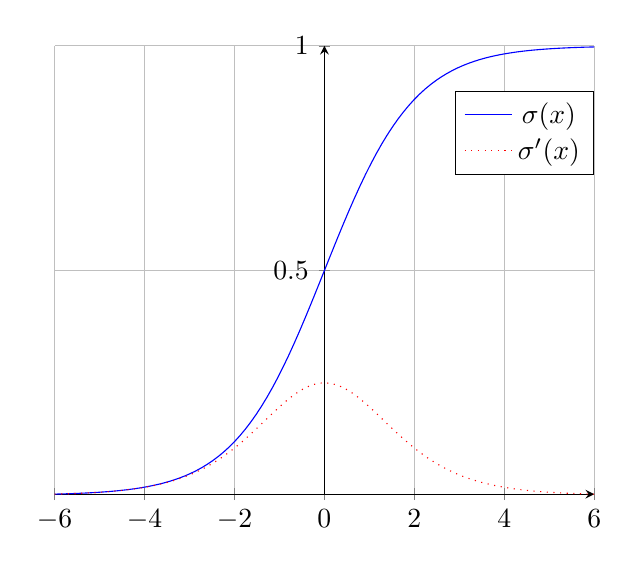
\begin{tikzpicture}[declare function={sigma(\x)=1/(1+exp(-\x));
sigmap(\x)=sigma(\x)*(1-sigma(\x));}]
\begin{axis}%
[
    grid=major,     
    xmin=-6,
    xmax=6,
    axis x line=bottom,
    ytick={0,.5,1},
    ymax=1,
    axis y line=middle,
    samples=100,
    domain=-6:6,
    legend style={at={(1,0.9)}}     
]
    \addplot[blue,mark=none]   (x,{sigma(x)});
    \addplot[red,dotted,mark=none]   (x,{sigmap(x)});
    \legend{$\sigma(x)$,$\sigma'(x)$}
\end{axis}
\end{tikzpicture}
\caption{A plot of a sigmoid activation function $\sigma(x)$ and its derivative $\sigma '(x)$.} \label{sigmoid:chart}
\end{figure}

A \emph{sigmoid function}, also referred to as sigmoid curve or logistic function (see figure \ref{sigmoid:chart}) is a function defined by the formula:

\begin{equation}
\sigma(x) = \frac{1}{1-e^{-x}}.
\end{equation}

While the sigmoid function was one of the first activation functions used in neural networks, its modern applications are limited due to a \emph{vanishing gradient} problem. For very high or very low values of $\sigma(x)$, its derivative's $\sigma '(x)$ values are small, causing equally marginal change of weights in the first layers of a model. Computing a value of sigmoid function also requires significantly more processing power as opposed to the \emph{ReLU} function.


\subsubsection{Rectified Linear Activation Unit}

\emph{Rectified Linear Activation Unit} (or ReLU) is an activation function defined as:

\begin{equation}
f(x) = max(0, x) = \begin{cases}
    x & \text{if } x > 0, \\
    0 & \text{otherwise}.
\end{cases}
\end{equation}

It is one of the most commonly used activation functions in modern deep learning models \cite{relu_def} due to the fact that the value of ReLU function can be easily computed. An \emph{ImageNet} image classification neural network has been shown to converge over 25\% faster when ReLU was used instead of $tanh$ function, for instance \cite{relu_speed}.

Being a differentiable function, ReLU allows the \emph{backpropagation} algorithm to be used during the process of training a neural network.

\begin{figure}
\centering
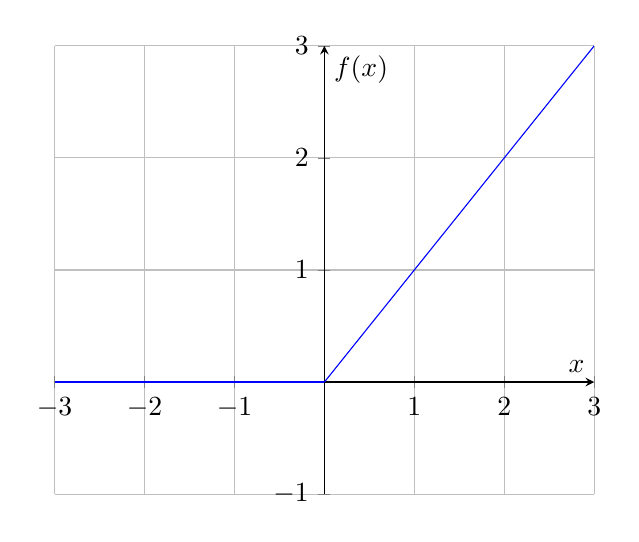
\begin{tikzpicture}
\begin{axis}[
    grid=major,     
    axis lines = middle,
    xlabel = $x$,
    ylabel = {$f(x)$},
    xmax = 3,
    xmin= -3,
    ymax = 3,
    ymin = -1,
    axis y line=middle,
    samples=100,
    domain=-3:3,
]
%Below the red parabola is defined
\addplot [
    domain=0:3, 
    samples=100, 
    color=blue,
]
{x};
\addplot [
    domain=-3:0, 
    samples=100, 
    color=blue,
]
{0};
 
\end{axis}
\end{tikzpicture}
\caption{A Rectified Linear Activation Unit is one of the most often used activation functions in modern neural networks.}
\end{figure}

\subsubsection{Softmax}

\emph{Softmax} is a function that takes as an input a vector of $K$ real numbers and normalises it into a probability distribution consisting of $K$ probabilities proportional to the exponential of the input numbers \cite{wiki:softmax}. It is defined as:

\begin{equation}
\sigma(\mathbf{z})_i = \frac{e^{z_i}}{\sum_{j=1}^K e^{z_j}} \text{ for } i = 1, \dotsc , K \text{ and } \mathbf z=(z_1,\dotsc,z_K) \in\mathbb{R} ^K,
\end{equation}

where on each element $z_i$ of an input vector $\textbf{z}$ a standard exponential function is applied and the calculated value is normalised through a division by the sum of all the exponents, ensuring that the sum of output vector's components $\sum_{i=1}^K\sigma(\mathbf{z})_i$ is equal to 1 and all the components of $\sigma(\mathbf{z})$ are in the range of $(0, 1)$. What's more, a relation between the value of an input and output probability is maintained - larger input components correspond to larger probabilities, and so forth.

Softmax is used as an activation function in neural networks to convert the outputs of neurons from a given layer into probability values, corresponding for instance to model's certainty that the input belongs to a given class in a classification problem.

\subsection{Hyperparameters}

\emph{Hyperparameters} in the context of neural networks are all the parameters of a given network which value is set before the beginning of a learning process.

They can be classified as model hyperparameters, which, in the context of neural networks include a number of hidden layers in a neural network, an amount of neurons per hidden layer and activation functions used in neurons, or algorithm hyperparameters, which affect the speed and outcomes of the learning process, such as the learning rate or mini-batch size \cite{wiki:hyperparams}.

\subsection{Backpropagation}

\emph{Backpropagation} method is an algorithm used during the training process of a neural network to calculate the changes of neuron weights and biases needed to be applied in order to minimise a given cost function, and thus improve an accuracy of the model.

The method's efficiency has allowed an application of neural networks to a much wider field of problems, that were previously off-limits due to time and cost constraints, due to its ability to produce internal representations of data on par with those manually-engineered, or even those found in biological neural networks \cite{backpropagation_brilliant}.

\subsubsection{Notation}

We use $w_{j, k}^l$ to denote the weight for the connection from the $k^{th}$ neuron in the $(l-1)^{th}$ layer to the $j^{th}$ neuron in the $l^{th}$ layer.

For the network biases, we denote $b_j^l$ as the bias of the $i^{th}$ neuron in the $l^{th}$ layer of the network, and for activations, we use $a_j^l$ for the activations of the $j^{th}$ neuron in the $l^{th}$ layer.

The activation $a_j^l$ of the $j^{th}$ neuron in the network is related to the activations in the $(l-1)^{th}$ layer by the equation

\begin{equation}
\label{notation:1}
a_j^l = \sigma(\sum_k w^l_{j, k}a^{l-1}_k + b_j^l),
\end{equation}
where the sum is over all neurons $k$ in the $(l-1)^{th}$ layer. 

In order to rewrite the expression \ref{notation:1} in a matrix form, the \emph{weight matrix} $\boldsymbol{w^l}$ is defined for each layer $l$, which is populated by weights connecting to the $l^{th}$ layer of neurons, which means, that the entry in the $j^{th}$ row and $k^{th}$ column is $w_{j, k}^l$. Similarly, for each layer $l$ a bias vector $\boldsymbol{b^l}$ is defined, which components are defined as $b^l_j$ values.

Having these matrices defined, the equation \ref{notation:1} can be rewritten as

\begin{equation}
\label{notation:2}
a^l = \sigma(w^la^{l-1}+b^l),
\end{equation}
which means, that in order to calculate the activations of neurons in one layer, all we have to do is to apply the weight matrix to the activations from a previous layer, then add the bias vector, and, finally, apply the $\sigma$ activation function. We also define

\begin{equation}
\label{notation:3}
\boldsymbol{z^l} \equiv w^la^{l-1} + b^l
\end{equation}
where $\boldsymbol{z^l}$ is called the \emph{weighted input} to the neurons in layer $l$ \cite{backpropagation_nielsen}.

\subsubsection{Cost function assumptions}

In order for the backpropagation method to be applied, we need to assume that our cost function $C$ can be expressed as an average $C = \frac{1}{n}\sum_x C_x$ over cost functions $C_x$,where $x$ is an individual training example. This is due to the fact that backpropagation allows us to compute partial derivatives $\frac{\delta C_x}{\delta w}$ and $\frac{\delta C_x}{\delta b}$, which $\frac{\delta C}{\delta w}$ and $\frac{\delta C}{\delta b}$ are recovered from by averaging over training examples. We will also assume for now that the training example $x$ is fixed, and refer to the cost $C_x$ as $C$, until otherwise noted.

We also need to make an assumption that a cost function can be expressed as a function of the outputs from a neural network $C = C(\boldsymbol{a^L})$. For example, a quadratic cost function $C = \frac{1}{2n} \sum_x ||y(x) - \boldsymbol{a^L}(x)||^2$ for a single training example $x$ may be written as :

\begin{equation}
\label{assumptions:1}
C = \frac{1}{2}||y-\boldsymbol{a^L}||^2 = \frac{1}{2} \sum_j (y_j - a_j^L)^2,
\end{equation}
and thus is a function of the output activations. While the function also depends on the desired output $y$, it's important to remember that both the training example $x$ and $y$ are fixed, and as such it is sound to regard $C$ as a function of $\boldsymbol{a^L}$, where $y$ is merely a parameter helping to define $C$ \cite{backpropagation_nielsen}.

\subsubsection{Hadamard product}

Let's suppose that $\boldsymbol{s}$ and $\boldsymbol{t}$ are two vectors of the same dimension. An \emph{element-wise} product of two vectors, also known as the \emph{Hadamard product}, is denoted as $\boldsymbol{s} \odot \boldsymbol{t}$, where: 
\begin{equation}
\label{hadamard:1}
(\boldsymbol{s} \odot \boldsymbol{t})_j = s_jt_j.
\end{equation}
\subsubsection{Backpropagation algorithm}

The backpropagation algorithm provides a way to compute a gradient of the cost function:

\begin{enumerate}
\item \textbf{Input} x: set the corresponding activation $a^1$ for the input layer
\item \textbf{Feedforward}: for each $l = 2, 3, \dots, L$ compute $\boldsymbol{z^L} = \boldsymbol{w^l}\boldsymbol{a^{l-1}} + \boldsymbol{b^l}$ and $\boldsymbol{a^l} = \sigma(\boldsymbol{z^l})$
\item \textbf{Output error} $\boldsymbol{\delta^L}$: compute the vector $\boldsymbol{d^L} = \Delta_a C  \odot \delta'(\boldsymbol{z^L})$
\item \textbf{Backpropagation of the error}: for each $l = L - 1, L - 2 \dots, 2$ compute $\boldsymbol{\delta^l} = ((\boldsymbol{w^{l+1}})^T \delta^{l+1}) \odot \sigma'(\boldsymbol{z^l})$ 
\item \textbf{Output}: the gradient of the cost function, given by $\frac{\delta C}{\delta w^l_{j, k}} = \boldsymbol{a^{l-1}_k \delta^l_j}$ and $\frac{\delta C}{\delta b_j^l} = \boldsymbol{\delta^l_j}$
\end{enumerate}

An error vector $\boldsymbol{\delta^j}$ is computed starting from the final layer, which is a consequence of the fact that the cost is a function of outputs from the network. The chain rule is applied repeatedly to evaluate the cost variations with weights and biases from earlier layers in the network \cite{backpropagation_nielsen}.

\subsection{Training neural networks}

% TODO: Verify and add that mini-batch gradient descent is a batch normalization

In order to train a neural network, the backpropagation method is combined with a learning algorithm, such as the mini-batch gradient descent, in order to compute a gradient of the cost function for many training examples.

\subsubsection{Mini-batch gradient descent-based backpropagation algorithm}

Given a mini-batch of $m$ training examples:

\begin{enumerate}
\item For each training example $x$: set the corresponding activation $a^{x, 1}$ and perform:        \begin{itemize}
  \item \textbf{Feed-forward}: for each $l = 2, 3, \dots, L$ compute $\boldsymbol{z^{x, L}} = \boldsymbol{w^l}\boldsymbol{a^{x,l-1}} + \boldsymbol{b^l}$ and $\boldsymbol{a^{x,l}} = \sigma(\boldsymbol{z^{x,l}})$
  \item \textbf{Output error} $\boldsymbol{\delta^{x, L}}$: compute the vector $\boldsymbol{d^{x, L}} = \Delta_a C_x  \odot \delta'(\boldsymbol{z^{x, L}})$
  \item \textbf{Backpropagation of the error}: \\ for each $l = L - 1, L - 2 \dots, 2$ compute $\boldsymbol{\delta^{x, l}} = ((\boldsymbol{w^{l+1}})^T \delta^{x, l+1}) \odot \sigma'(\boldsymbol{z^{x, l}})$
  \end{itemize}
\item \textbf{Gradient descent}: for each $l = L, L - 1, \dots, 2$ update 
\begin{itemize}
    \item weights, according to the rule $w^l \rightarrow w^l - \frac{\eta}{m} \sum_x \delta^{x,l} (a^{x, l - 1})^T$
    \item biases, according to $b^l \rightarrow b^l - \frac{\nabla}{m} \sum_x \delta^{x, l}$.   
\end{itemize}
\end{enumerate}

An implementation of stochastic gradient descent will also require two outer loops, one generating mini-batches of $m$ training examples and another iterating over multiple epochs of training, which were omitted for simplicity \cite{backpropagation_nielsen}.

\subsection{Regularisation}

In order to reduce overfitting in neural networks, a set of methods known as \emph{regularisation} techniques has been developed in order improve the generalisation from the training data to the test data. An example of such an technique is a \emph{L2 regularisation} method \cite{backpropagation_nielsen}.

\subsubsection{L2 regularisation}

\emph{Weight decay}, also known as the L2 regularisation, is one of the most commonly used regularisation techniques, which works by adding an extra term to the cost function $C$ - the sum of all squared weights in the neural network:

\begin{equation}
C = C_0 + \frac{\lambda}{2n} \sum_w w^2,
\end{equation}
where $C_0$ is the unmodified cost function, $\lambda > 0$ is an \emph{regularisation parameter}, and $n$ - the size of a training set. A quadratic cost function with L2 regularisation applied is defined then as follows: 

\begin{equation}
C = \frac{1}{2n} \sum_x ||y - a^L||^2 + \frac{\lambda}{2n} \sum_w w^2,
\end{equation}
For small values of $\lambda$, the regularisation has an effect of minimising the original cost function, and for the large values of $\lambda$ - affects the values of the network's weights, making it preferred to learn smaller values \cite{backpropagation_nielsen}.

\begin{figure}[]
\centering
\includegraphics[scale=0.48]{figures/regularisation.png}
\caption{Regularisation helps trained models to generalise better to new data by limiting the complexity of the model caused by an overfitting to the noise in the training data. An example of underfitting, a good bias-variance trade-off and overfitting is shown here accordingly in plots depicting a degree 1-, 4- and 15- polynomial attempting to match the training samples given \cite{regularisation_scikit}.}
\end{figure}

\subsubsection{Dropout}

Arguably the most popular regularisation technique for neural networks is known as \emph{dropout}. Introduced in 2012, it has proven to improve the accuracy of state-of-the-art models by 1-2\%, decreasing their error rate by almost 40\% \cite{handson_geron}.

Dropout works by assigning each neuron in the neural network excluding an output layer a new hyperparameter, which is the probability $p$ (most often set to $p = \frac{1}{2}$) of a neuron being omitted during a single training step. After the training, the neurons are no longer excluded from the computations.

Applying such an omission during training has been shown to produce subsequent data representations by neurons which contribute towards the solution of a given task, instead of representations helpful only in context of several other feature detectors. This has an effect of training multiple training networks with different hyperparameters and then averaging their output to produce a final output - but is much more computationally efficient \cite{dropout}. 

\section{Deep learning}

\emph{Deep learning} is a subset of machine learning methods focusing on learning representations of data, often expressed in terms of other, simpler representations, which aim is to solve a given target task \cite{goodfellow}. Its approach to the problem of representation learning has proven to be effective in solving problems perceived as difficult in the fields of computer vision and natural language processing, among others.

% Some more background on deep learning needs to go there

Most modern deep learning solutions are based upon \emph{deep neural networks}.

\subsection{Deep neural networks}

Deep neural networks are machine learning models which utilise multiple hidden layers in their internal infrastructure in order to produce a highly accurate representations of data.

\subsection{Recurrent neural networks}
\label{rnns}

\emph{Recurrent Neural Networks} (or \emph{RNNs}) are neural networks which work on arbitrary-length sequences as opposed to fixed-size inputs. The input sequences are processed by iterating through their elements and maintaining a \emph{hidden state} containing information relative to what's been already processed \cite{chollet}.

RNNs are used in natural language processing tasks such as text translation or sentiment analysis, \emph{time series} analysis and content generation \cite{rnn_generation}. Unlike feedforward neural networks, RNNs have connections pointing backwards.

\subsubsection{Memory cells}

\emph{Memory cells} are basic building blocks of recurrent neural networks. At an each time step $t$ a single memory cell outputs its hidden state $h_{(t)}$, which is a function of an input at that time step and the cell's state at the previous time step

\begin{equation}
h_{(t)} = f(h_{(t-1}, x_{(t)}).
\end{equation}

The cell's output at time step $t$, denoted as $y_{(t)}$ is also a function of the previous state and current inputs.

\begin{figure}[]
\centering
\includegraphics[scale=0.6]{figures/memory_cells.png}
\caption{Memory cell's hidden state $h_{(t-1)}$ is passed as an input to the cell at the time step $t$, allowing the cell to take account its previous inputs when producing an output $y_{(t)}$. A recurrent cell can be \emph{unrolled}, which means, that it is represented against a time axis, as shown in this example \cite{handson_geron}. }
\end{figure}

\subsubsection{Long Short-Term Memory Cell}
\label{lstm}

\emph{Long Short Term Memory Cell} (or \emph{LSTM}) is a memory cell whose internal state is split into two vectors: $h_{(t)}$, representing a short-term state, and $c_{(t)}$, which represents a long-term state \cite{lstm_cell}. 

\begin{figure}[]
\centering
\includegraphics[scale=0.9]{figures/lstm_cell.png}
\caption{A LSTM cell through an introduction of both a short-term and long-term state, allowing the neural network to take into account from different time steps $t_i$ depending on their determined importance  \cite{handson_geron}.}
\end{figure}

% ADD UNDER THE IMAGE AN EXPLAINATION OF INPUTS, OUTPUTS; maybe use another graphic which will depict the cell better

A RNN learns whether an information should be kept, removed or read from $c_{(t)}$ in a LSTM cell. At each time step $t$ an input long term state from a previous time step, $c_{(t-1)}$:

\begin{enumerate}
\item passes through a \emph{forget gate}, which controls what information should be removed from $c_{(t)}$,
\item has an addition operation performed on it based on the output of an \emph{input gate},
\item is returned as a long term state $c_{(t)}$ of the cell at a current time step.
\end{enumerate}

After the addition operation $c_{(t)}$'s state is copied and passed through a tanh function, which result is then modified by an \emph{output gate}. These operations produce a short-term state $h_{(t)}$ equal to the cell's output for a current time step, denoted as $y_{(t)}$.

Also, at each time step $t$ an input vector $x_{(t)}$ is passed along with $h_{(t-1)}$ through four fully-connected layers:

\begin{enumerate}
\item A layer outputting $g_{(t)}$, which is computed based on $x_{(t)}$ and $h_{(t-1)}$'s values,
\item A forget gate controller layer ($f_{(t)}$) controlling which parts of the long-term state to erase,
\item An input gate controller layer ($i_{(t)}$), which determines what parts of $g_{(t)}$'s output are added to $c_{(t)}$,
\item An output gate controller layer ($o_{(t)}$), determining which parts of $c_{(t)}$ should be output at $t$.
\end{enumerate}

The LSTM cell can be thus defined mathematically as:
\begin{equation}
\begin{split}
&i_t = \sigma(W^ix_t + U^ih_{t-1})\\
&f_t = \sigma(W^fx_t + U^fh_{t-1})\\
&o_t = \sigma(W^ox_t + U^oh_{t-1})\\
&g_t = tanh(W^cx_t + U^ch_{t-1})\\
&c_t = i_t \odot g_t + f_t \odot c_{t-1}\\
&h_t = o_t \odot tanh(c_t),\\
\end{split}
\end{equation}
where $W^i, W^f, W^o, U^i, U^f, U^o, U^c$ are weight matrices and $\odot$ is an element-wise multiplication.

\subsubsection{Backpropagation through time}

A recurrent neural network is trained using a strategy called the \emph{backpropagation through time} (or \emph{BPTT}), which is a regular backpropagation algorithm applied to a RNN unfolded through time.

\begin{figure}[]
\centering
\includegraphics[scale=0.9]{figures/bptt.png}
\caption{An illustration of the backpropagation through time strategy applied to an unfolded RNN. Note that the gradient is computed for all outputs used by the cost function (in this instance $Y_{2}$, $Y_{3}$ and $Y_{4}$), not just the final output of a network \cite{handson_geron}.}
\label{bptt:1}
\end{figure}

Similarly to previously discussed algorithm, the forward pass is performed through the unfolded RNN, represented in figure \ref{bptt:1} by the dashed arrows. Then, an output sequence is evaluated using a cost function:
\begin{equation}
C(Y_{(t_{min})}, Y_{(t_{min} + 1)}, \dots, Y_{(t_{max})}),
\end{equation}
where $t_{min}$ and $t_{max}$ represent first and final time steps, excluding ignored outputs, and the gradients of $C$ are propagated backward through the unrolled network (step marked in figure \ref{bptt:1} as solid arrows). The computed gradients are used to update the model's parameters $\theta$.

\chapter{Recurrent neural networks-based natural language processing and document sentiment classification} 
\label{chapter:rnnnlp}

Recurrent neural networks' ability to process arbitrary length inputs and interpret information based on a given context makes them an auspicious base for modern natural language processing systems. In fact, most of the state-of-the-art NLP applications, including document sentiment classification are based on RNNs \cite{handson_geron}.

However, this has not always been the case. Until 2013, recurrent neural networks had been thought to be difficult to train \cite{ruder:neuralnlp,sutskever:rnntraining} and most of the latter approaches required large datasets and prolonged computational time in order to converge \cite{ulmfit}. 

In this chapter we discuss some of the key milestones in the field of neural network-based natural language processing, which have resulted in addressing aforementioned shortcomings and proliferation of cutting-edge NLP solutions. We also explain core concepts behind modern NLP frameworks and tool-kits, such as \emph{tokenization}.

Finally, this chapter provides a perspective on the significance of introduced developments in the context of a task of document-level sentiment classification and the entire field of natural language processing. In this process, some of the established methods are introduced, including ULMFiT.

% Maybe write here that Google was able to cut down on their translation systems complexity, reducing the amount of code from 50,000 to 500 lines thanks to neural network-based NLP?

\section{Document representation}
\label{document:representation}

In order for a text document to be processed by a neural network it has to be converted into a numerical representation. Most often such a document is represented by a vector obtained through a process called \emph{text vectorization} \cite{chollet}.

\subsection{Tokenization}

Before a given text document can be vectorized, it has to be first segmented into individual subsequences, such as individual words, characters, or groups of multiple consecutive words or characters known as \emph{n-grams} \cite{chollet}. Such a task is referred to as \emph{tokenization}. 

Individual subsequences produced by a \emph{tokenizer}, a system performing the tokenization, are called \emph{tokens}. An example illustration of a tokenization process for a sentence in English is shown in a figure \ref{tokenization:1}. A set of all the tokens generated by the tokenizer is called a \emph{token vocabulary}, denoted as $V^*$.

\begin{figure}[]
\centering
\includegraphics[scale=0.5]{figures/tokenization.png}
\caption{An illustration of the tokenization process performed by a \emph{spaCy} tokenizer \cite{spacy:101}. A raw text (\textit{"Let's go to N.Y.!"})  is first split into subsequences on whitespace characters and for each subsequence a check is performed against a tokenizer's predefined set of rules and exceptions. Here, \textit{"Let's} is first split into \textit{"} and \textit{Let's} based on a prefix splitting rule. Then \textit{Let's} is again split into tokens \textit{Let} and \textit{'s} according to a defined exception (in English, \textit{Let's} is short for \textit{Let us}). Similarly, \textit{N.Y.!"} produces tokens \textit{N.Y.}, \textit{!} and \textit{"}. }
\label{tokenization:1}
\end{figure}

More advanced tokenization methods, such as \emph{Byte-Pair-Encoding segmentation} have been shown to increase a performance on many tasks, such as machine translation \cite{kudo:subword}. 

In highly inflected languages\footnote{Latin, Polish or Finnish are examples of highly inflected languages.} (see section \ref{sentiment:polish}) a properly chosen tokenization method helps to reduce the amount of tokens generated, increasing the model's ability to interpret their meaning without increasing the size of the vocabulary, having a positive impact on model's complexity, training duration and efficiency.

\subsection{One-hot encoding}

Tokens represent a discrete, categorical features, which can be represented as a vector through a method referred to as \emph{one-hot encoding} \cite{hirst:neuralnetworkmethodsinnlp}.

Using one-hot encoding, each token $t_i$ in the vocabulary of size $n$ is assigned an unique index $i \in \{0, 1, \dots, n-1\}$. Then, for each $t_i$, a vector $v$ of size $n$ is created, where all the elements are $0$, except for the $i$-th entry, which has a value of $1$.

Vectors obtained through one-hot encoding are binary, sparse and highly-dimensional, making them computationally inefficient for larger vocabularies. Such an encoding also does not maintain any semantic relationship between input tokens and output vectors, resulting in a loss of valuable information which could be taken advantage of during the process of training a neural network \cite{tds:embeddings}. Thus, another vectorization method called \emph{word embeddings} is more commonly used.

\subsection{Token embeddings}
\label{embeddings}

Token embeddings are an efficient, dense representation of tokens in which similar tokens have a similar encoding. An embedding is a dense vector of floating-point values, which are the weights learned during the process of training a neural network.

The dimensionality of token embeddings varies depending on the size of the dataset. The more dimensional the embeddings are, the more likely they are to depict relationships between used tokens, at a cost of requiring more training data in order to learn \cite{tf:embeddings}. 

% insert here a visual comparison between word embeddings and one-hot encoded vectors

\subsection{Token embeddings layer}

A \emph{token embeddings layer} is an input layer of a neural network that performs mapping from integer indices representing individual tokens to associated vector embeddings \cite{tf:embeddings,ulmfit}.

Depending on an implementation, an embeddings layer may use as an input an integer index $i \in \{0, 1, \dots, n-1\}$ assigned for each token $t$ in a vocabulary $V^*$ of size $n$ \cite{tf:embeddings} or a one-hot-encoded vector representation of $t$ \cite{ulmfit:berlin}.

% cite word2vec
% Compared to vectors obtained through a one-hot encoding method, token embeddings are usually learned during a supervised learning task. A choice of such a task is one of the key factors affecting their effectiveness \cite{tds:embeddings}.

\subsection{Notation and assumptions on words and tokens}

We will denote an individual word as $w$ and a word vocabulary as $V$. Similarly, an individual token will be denoted as $t$, and the vocabulary of tokens as $V^*$. Words always convey a particular meaning, while the tokens are an output of a tokenizer \cite{hirst:neuralnetworkmethodsinnlp}. The goal of tokens is to simplify a word and syntax-based meaning representation, through a generation of token-based representation.

For the purposes of simplicity, we will use the term words in the latter parts of this paper almost exclusively, unless it is important to make a distinction between them.

\subsection{Corpora transformations}

In natural language processing, a set of text documents used in a given learning task is referred to as \emph{corpus}. Corpus can be either labelled or unlabelled, depending on a machine learning task it's applied to.

In order to use a text corpus for the purposes of training a recurrent neural network, it's contents, after tokenization, needs to be concatenated into a single entity. Such a process requires an addition of two tokens: a token signifying the beginning of a concatenated document, $T_{\mathrm{BEG}}$, and a token put at the end of each concatenated document, $T_{\mathrm{END}}$. 

Defining $C$ as a corpus and $d_i$ as an individual member of the corpus, the resulting entity $e$ is created:

\begin{equation}
e =(T_{\mathrm{BEG}}\oplus d_1 \oplus T_{\mathrm{END}}) \oplus (T_{\mathrm{BEG}}\oplus d_2 \oplus T_{\mathrm{END}}) \oplus \dots (T_{\mathrm{BEG}} \oplus d_n \oplus T_{\mathrm{END}}),
\end{equation}

where $n$ is the length of the corpus (total number of text documents in a set) and $\oplus$ is the concatenation. 

\begin{figure}[]
\centering
\includegraphics[scale=0.45]{figures/minibatch.png}
\caption{In a mini-batch-based process of training a RNN, a concatenated entity $e$ of text documents is first split into a number of batches based on a defined batch size $bs$. As a result, batches consisting of $n_t$ tokens are created,  illustrated as a $bs \times n_t$ matrix. Then, mini-batches are created by truncating created batches based on a value of $bptt$ parameter, which indicates, how many tokens are going to be back-propagated through when training the model. For instance, having a mini-batch consisting of 64 sequences of 70 tokens, during the training one mini-batch is fed to the model, and, as a result, all 64 sequences are processed in parallel. For each mini-batch model performs its predictions and calculates the loss before a backpropagation process begins \cite{ulmfit:berlin}.}
\label{corpus:minibatch}
\end{figure}

However, due to computational and memory constraints, training a RNN using a large corpora is performed using a mini-batch-based backpropagation through time algorithm (see figure \ref{corpus:minibatch}) \cite{ulmfit:berlin}.

% \section{Language modelling}
% \label{languagemodelling}

% \emph{Language modelling} is the task of learning a probability distribution over words in a given vocabulary $V$. As a result, a language model is created, which assigns probability for the likelihood of a given word (or sequence of words) to follow an arbitrary sequence of words \cite{hirst:neuralnetworkmethodsinnlp}.

% Most often the aim of the language models is to compute the probability of the occurrence of word $w_t$ given $n-1$ previous words in a sequence, denoted as $P(w_t | w_{t-1}, w_{t-2}, \dots, w_1)$, where \cite{ruder:onwordembeddings}:

% \begin{equation}
% P(w_t | w_{t-1}, w_{t-2}, \dots, w_1) = P(w_1) P(w_2 | w_1)P(w_3|w_1w_2)\dots P(w_t|w_1w_2\dots w_t-1).
% \label{lm_1}
% \end{equation}

% Due to the fact that the last term of equation \ref{lm_1} requires conditioning on $n - 1$ words, which is a task almost equally difficult as modelling an entire sentence, language models rely on the \emph{Markov assumption}, assuming that the next word in a sequence depends only on the last $k$ words (\textit{"future is independent of past given the present"}) \cite{hirst:neuralnetworkmethodsinnlp}:

% \begin{equation}
% P(w_i |w_{i-1} w_{i-2}\dots w_{1}) \approx P(w_i |w_{i} w_{i-1}\dots w_{i-k}).
% \end{equation}

% The probability of a whole sentence or a document can be as such approximated by the product of probabilities of each word given $n$ previous words \cite{ruder:onwordembeddings}:

% \begin{equation}
% P(w_1, w_2, \dots, w_t) = \prod_i P(w_i | w_{i-1} w_{i-2} \dots w_{i-n+1}).
% \end{equation}
% % should I add that in neural networks softmax is used for this? https://ruder.io/word-embeddings-1/index.html#classicneurallanguagemodel

\section{Transfer learning: from fine-tuning of pre-trained word embeddings to fine-tuning of pre-trained language models}

Most of the earlier research on transfer learning applications in neural network-based natural language processing focused on transductive transfer learning, where, for instance, the models' ability to perform accurate predictions in classification tasks when documents from a different domain were used as an input was measured \cite{transductive:blitzer,ulmfit}. 

For inductive transfer learning, two noteworthy techniques have been proposed: first, a fine-tuning of pre-trained word embeddings method was proposed \cite{word2vec}, and later - fine-tuning of entire, pre-trained models \cite{ulmfit}.

\subsection{Fine-tuning pre-trained word embeddings}
\label{finetuning:embeddings}

In order to improve the word embeddings' ability to represent semantic relationships between words in a given vocabulary $V$, highly-specialised machine learning models, such as \emph{word2vec} and \emph{GloVe} have been used, which, due to a substantial improvement of their performance, have allowed to be trained on much larger datasets, thus obtaining relation-maintaining word embeddings \cite{embeddings:relations,word2vec,glove}. 

Applied in an embedding layer of a neural network, pre-trained word embeddings have been shown to increase the model's performance on various NLP tasks \cite{embeddings:accuracy,embeddings:accuracy2}.

However, as the usage of pre-trained word embeddings affects only the first layer of a model, the remaining parameters still remain randomly initialised. Taking into account the benefits of pre-training an entire model, which include an improved generalisation \cite{pretraining:benefits}, first successful language model pre-training and fine-tuning methods have been proposed. Their impact on neural networks-based natural language processing cannot be understated \cite{state_of_nlp_2019}.

%TODO: Add word vectors illustration

\subsection{Fine-tuning pre-trained language models}
\label{finetuning:languagemodels}

Language models had been historically thought to be prone to suffering from a phenomena known as \emph{catastrophic forgetting} \cite{goodfellow:forgetting} when fine-tuned with a classifier, as well as requiring large datasets in order not to overfit \cite{dai:sequencelearning}. Nowadays, they are ubiquitous in natural language processing, allowing for state-of-the-art results to be achieved on a wide range of tasks \cite{state_of_nlp_2019}. 

This is due to the fact that novel methods, such as the ULMFiT \cite{ulmfit}, \emph{BERT} \cite{bert} or \emph{GPT2} \cite{gpt2} have made it possible to perform a successful pre-training and latter fine-tuning of a deep neural networks-based language model.

Language modelling as a pre-training source task has also been shown to lead to a better performance on target task, as opposed to machine translation or auto-encoding \cite{languagemodels:vstranslation}, especially when syntactic information is of relevance.

\begin{figure}[]
\centering
\includegraphics[scale=0.33]{figures/ulmfit_results.png}
\caption{A comparison of validation error rates for supervised and semi-supervised ULMFiT method applications as opposed to training an AWD-LSTM model from scratch, with varying amount of training examples. Tests were performed on \emph{IMDB} (left), \emph{TREC-6} (center) and \emph{AG} (right) datasets  \cite{ulmfit}.}
\label{ulmfit:results}
\end{figure}

Arguably, the most important benefit of using a pre-trained language model is that it substantially reduces the amount of labelled training examples needed for a target model to converge, as shown in figure \ref{ulmfit:results}. It is, however, computationally expensive to pre-train a language model which reaches a low \emph{perplexity}\footnote{Perplexity is a measurement of how well a probability distribution or probability model predicts the sample. The perplexity of language model can be understood as the level of perplexity when predicting the following word - a total number of choices a language model can make \cite{perplexity}.} which is a measurement of how well a probability distribution or probability model predicts a sample \cite{state_of_nlp_2019}.

\section{AWD-LSTM}
\label{awdlstm}

Due to over-parametrisation of neural networks, their generalisation ability depends heavily on the regularisation techniques used. However, naive applications of strategies, such as dropout and batch normalisation in recurrent neural networks have not been highly successful, compared to results in feed-forward and convolutional neural networks. 

A proposal of \emph{AvSDG Weight-Dropped LSTM} (or \emph{AWD-LSTM}), a set of regularisation strategies developed for RNNs \cite{merity:awdlstm} has helped to produce state-of-the-art results in language modelling \cite{ulmfit:berlin}.

\begin{table}[ht]
\centering
\begin{tabular}{ lcc }
\toprule
Model & Validation & Test \\ \midrule
AWD-LSTM & 68.6 & 65.8 \\ \midrule
- variable sequence lengths & 69.3 & 66.2 \\
- embedding dropout & 71.1 & 68.1 \\
- weight decay & 71.9 & 68.7 \\
- AR/TAR & 73.2 & 70.1 \\
- weight-dropping & 78.4 & 74.9 \\ 
\bottomrule
\end{tabular}
\caption{An impact of removal of regularisation techniques used in AWD-LSTM on the model's validation and test perplexity measured on a \emph{WikiText-2} dataset. A removal of hidden-to-hidden weights regularisation performed by weight dropping alone leads to an increase of over 10 points of perplexity as compared to a model employing all the regularisation strategies, proving that regularisation has a significant, positive impact on the recurrent neural network's performance \cite{merity:awdlstm}.}
\end{table}

\subsection{Weight-dropped LSTM}
\label{weightdropped}

AWD-LSTM makes use of \emph{DropConnect} on the recurrent, hidden-to-hidden weight matrices ($U^i, U^f, U^o, U^c$), as opposed to previous techniques, which introduced dropout between time steps, acting on hidden state vector $h_{t-1}$, or on update of a memory state $c_t$.

\begin{figure}[]
\centering
\includegraphics[scale=0.6]{figures/dropconnect.png}
\caption{DropConnect sets a randomly selected subset of weight values in a neural network to zero, as opposed to a regular droput, which is applied as a mask, denoted here as $m(\cdot)$, on a random subset of network's activations $a(\cdot)$ \cite{dropconnect}.}
\label{dropconnect}
\end{figure}

This enables the use of external, highly-optimised LSTM implementations, such as \emph{cuDNN LSTM} \cite{merity:awdlstm}, while retaining the LSTM's ability to learn long term dependencies of input data \cite{seth:awdlstmgreat}.

\subsection{Variable-length backpropagation through time}
\label{vl:bptt}

Having a fixed length of sequences in a mini-batches used to train the network using the backpropagation through time algorithm results in an inefficient use of available training data. Merity et al. illustrates this by an example: having 100 elements to perform a backpropagation with a fixed $bptt$ window of 10, any element divisible by 10 will not have any element to backpropagate into \cite{merity:awdlstm}, essentially meaning, that for an every final element of a mini-batch a language model's prediction is never performed. To prevent such an inefficiency, an use of \emph{variable-length backpropagation sequences} was proposed. 

Using variable-length backpropagation sequences approach, a base sequence length is determined to be $bptt$ with probability $p$ and $\frac{bptt}{2}$ with probability $1-p$. Then, a sequence length $l$ is selected according to $\mathcal{N}(bptt, s)$, where $s$ is the standard deviation and $\mathcal{N}$ - a normal distribution \cite{seth:awdlstmgreat}. This results in a more efficient usage of available training data.

\subsection{Variational dropout}
\label{variationaldropout}

\emph{Variational dropout} addresses the inefficiency of applying a regular dropout in long short-term memory networks, by performing a generation of a dropout mask once and then re-using a generated mask within a single forward and backward pass, as opposed to its re-generation on every dropout function call . This ensures that in an RNN at each time step $t$ an identical dropout mask is applied for input $x_t$. 

In AWD-LSTM, variational dropout is used in all dropout operations, excluding those related to hidden-to-hidden weight matrices described in section \ref{weightdropped}. Specifically, a variational dropout mask is applied for all inputs and outputs of LSTM \cite{merity:awdlstm}.

\subsection{Embeddings dropout}
\label{embeddingsdropout}

Another regularisation called \emph{embeddings dropout} is used in AWD-LSTM to perform a dropout on a randomly-chosen set of inputs to the embedding matrix of a neural network, resulting in some of the input tokens being omitted during a single forward and backward pass process of training a network.

Intuitively, the goal of using an embeddings dropout is to make a model less prone produce output based on the presence of individual tokens. Used with variational dropout, embeddings dropout method has been shown to improve the performance of LSTM-based natural language processing models performing language modelling \cite{merity:awdlstm} and sentiment analysis \cite{gal:embeddingdropout}, among others.

\subsection{Activation regularisation and temporal activation regularisation}

An \emph{activation regularisation} is a L2 regularisation applied to the individual activation values of the neural network in order to penalise activations significantly larger than 0 as a mean of regularising the network. It is defined as:

\begin{equation}
AR = \alpha \cdot {L2}(m \odot h_t),
\end{equation}

where $m$ is the dropout mask, $h_t$ is the output of the recurrent neural network at timestep $t$ and $\alpha$ is a scaling coefficient. 

To prevent substantial changes between hidden state values at subsequent time steps, a \emph{temporal activation regularisation} is used:

\begin{equation}
TAR = \beta \cdot L2(h_t - h_{t+1}),
\end{equation}

where $\beta$ is a scaling coefficient. Both TAR and AR are applied only to the output of the final RNN's layer \cite{merity:regularisations,merity:awdlstm}.

\section{Adam optimiser}
\label{adam:optimiser}

Gradient descent-based optimisation methods are by far the most common way to optimise neural networks. However, an usage of plain mini-batch gradient descent algorithm (introduced in section \ref{gradient:mini-batch}) is not ideal due to the fact that it is often difficult to choose a proper learning rate: small $\eta$ leads to a slow convergence, while high $\eta$ might cause the loss function to fluctuate around its local/global minimum, or even to diverge.

An \emph{Adaptive Moment Estimation} (or \emph{Adam}) is a SDG-based method that computes adaptive learning rates for each parameter \cite{adam:paper}. In Adam, an exponentially decaying average of past gradients, denoted as $m_t$:
\begin{equation}
m_t = \beta_1 m_{t-1} + (1 - \beta_1) g_t,
\end{equation}

which estimates the first moment of the gradient (the mean) is stored, along with an exponentially decaying average of past squared gradients, defined as $v_t$:

\begin{equation}
v_t = \beta_2 v_{t-1} + (1 - \beta_2)g_t^2,
\end{equation}

estimating the second moment (the uncentered variance) of the gradient \cite{ruder:sdgsadam}. 

It has been observed that both $m_t$ and $v_t$ initialised as vectors of zeros are biased towards zero, especially during the initial time steps, and when the decay rates are small ($\beta_1$ and $\beta_2$ are close to zero). To counteract this bias, bias-corrected first and second moment estimates are computed:

\begin{equation}
\begin{split}
\hat{m_t} = \frac{m_t}{1 - \beta_1^t},\\
\hat{v_t} = \frac{v_t}{1 - \beta_2^t},\\
\end{split}
\end{equation}

in order to be used to update the parameters of the model \cite{ruder:sdgsadam}:

\begin{equation}
\theta_{t+1} = \theta_t - \frac{\eta}{\sqrt{\hat{v_t}} + \epsilon} \hat{m_t}.
\end{equation}

An usage of default parameters of $\beta_1 = 0.99$, $\beta_2 = 0.999$ and $\epsilon = 10^{-8}$ has been proposed by authors of the method \cite{adam:paper}.

\begin{figure}[]
\centering
\includegraphics[scale=0.30]{figures/hbf.png}
\caption{Adam is an example of a \emph{Heavy Ball with Friction} (\emph{HBF}) method. It's averaging over past gradients corresponds to a velocity that results in the optimiser being "resistant" to be pushed into small regions. Adam has been shown to overshoot small, local minima of functions and be able to find flat minima which result in a improved generalisation of an optimised model, as shown in this illustration \cite{gans:adam}.}
\label{adam}
\end{figure}

\section{Impact on natural language processing}
\label{impact:nlp}

While different methods of pre-training word embeddings have been extensively used in many deep learning-based NLP models with an effect of improved performance by 2-3 percentage points \cite{kim:cnnembeddings}, they have been able to affect only embedding layers of neural networks, leaving the majority of network parameters randomly initiated \cite{ulmfit}. 

This requires a model using word embeddings not only to learn from scratch how to disambiguate words, but also how to derive meaning from a sequence of words, modelling complex phenomena such as \emph{compositionality}\footnote{The principle of compositionality is the principle that the meaning of a complex expression is determined by the meanings of its constituent expressions and the rules used to combine them \cite{wiki:compositionality}.}, \emph{polysemy}\footnote{Polysemy is the capacity for a word or phrase to have multiple meanings, usually related by contiguity of meaning within a semantic field \cite{wiki:polysemy}.}, \emph{anaphora}\footnote{Anaphora is the use of an expression whose interpretation depends upon another expression in context \cite{wiki:anaphora}.}, long-term depedencies, agreement, negation, and many more core aspects of natural language understanding \cite{ruder:nlpimagenetmoment}. As a result, the model's performance still depends on a large set of training examples available, limiting usefulness of the method when task-specific data sources are scarce.

An emergence of \emph{ELMo} \cite{peters:elmo}, ULMFiT \cite{ulmfit} or \emph{OpenAI transformer} \cite{openai:transformer} among others has radically changed the NLP landscape, successfully demonstrating that pre-trained language models can be used to achieve state-of-the-art results in the field. The impact of a paradigm shift from using pre-trained word embeddings to pre-trained language models has been as significant to the field of natural language processing as the introduction of models pre-trained on ImageNet \cite{imagenet:dataset} for computer vision \cite{ruder:nlpimagenetmoment}, resulting in a substantial improvement of target models' performance \cite{henaff:contrastivepredictivecoding,state_of_nlp_2019}. In case of ULMFiT, over ten times less labelled examples are needed for the target classifier model to achieve similar performance to a non-pre-trained model (see \autoref{ulmfit:results}) \cite{ulmfit}.

It would not be possible for language models to make such an impact on the machine learning-based NLP field if it weren't for improvements in the area of tokenization (\autoref{document:representation}), neural network regularisation, and optimisation, among others. For instance, ULMFiT relies heavily on the work of Merity et al. on AWD-LSTM (\autoref{awdlstm}), implementing its regularisation strategies, as well as Adam stochastic optimisation (\autoref{adam:optimiser}).

Latest pre-training methods, such as \emph{RoBERTa} \cite{liu:roberta} or \emph{MultiFiT} \cite{howard:multifit} prove that the performance of language modelling can be still performed through an experimentation with different neural network infrastructures, amount of unsupervised training data, cross-lingual language modelling, and more \cite{state_of_nlp_2019}.

\section{Impact on document-level sentiment classification}

When a neural networks-based model is used in a natural language processing task, including the domain-level sentiment classification, it is required for a model to obtain knowledge about the language, ranging from low-level (such as meaning of words) to high-level (e.g. that the dog barks) \cite{raffel:limitsoftransferlearning}.

Such a knowledge can be obtained by training a neural network on a large set of domain-specific documents for a given target task. Unfortunately, obtaining high accuracy this way has often involved datasets consisting of tens of thousands, if not hundreds of thousands of in-domain documents. This has proven to limit neural networks-based NLP applications to tasks with relatively large amount of labelled training data available \cite{ulmfit}. For a problem of document-level sentiment classification, such a requirement has limited neural networks-based implementations to languages, such as English, for which a vast amount of qualitative opinion sources, including \emph{Amazon} or {IMDB} reviews could be found.

An advent of methods for inductive transfer learning-based pre-training and fine-tuning of language models has, however, fundamentally changed the NLP landscape, leveraging widely available, unlabelled sets of textual information in virtually every language, such as Wikipedia, as means of learning both low-level and high-level representations of data (see section \ref{impact:nlp}).

ULMFiT, being a notable example such a technique, utilises LSTM recurrent neural networks-based language models (section \ref{rnns}) with applied AWD-LSTM regularisation techniques, such as variational dropout, weight-dropped LSTM or embeddings dropout (section \ref{awdlstm}), used in an inductive transfer learning process (section \ref{transferlearning:inductive}) of domain-general dataset-based language model pre-training, and latter, domain-specific dataset-based language model fine-tuning (see section \ref{finetuning:languagemodels}) and final training to produce a text classifier, which achieves performance comparable to training an entire RNN model from scratch while requiring up to twenty times less labelled training data \cite{state_of_nlp_2019,ulmfit}.

As such, a language model-based document sentiment classification system pre-trained on general, unlabelled data (such as encyclopedic documents), fine-tuned on domain-specific unlabelled opinions (often easier to find in greater amounts than labelled ones), and finally trained on just thousands of target labelled opinion examples, can achieve a high overall performance of over 95 \% on less than 10000 labelled examples \cite{raffel:limitsoftransferlearning,lan:albert,liu:roberta,liu:mtdnn}. This means that by leveraging language model pre-training and fine-tuning, neural networks-based document sentiment classification can be performed on a variety of new languages and domains, previously limited by scarcity of available labelled data.

An additional benefit of using pre-trained language models is that, once trained, they can be re-used for a wide variety of NLP tasks from different domains. Having pre-trained a Polish domain-general language model on a set of Wikipedia documents, we can use it for purpose of numerous NLP tasks, including document sentiment analysis and any text classification. When a goal is to prepare separate document sentiment classifiers for a variety of Polish product review sources (e.g. Filmweb, Allegro, Empik), a previously prepared domain-general language model can be fine-tuned on data available from all these sources, and then multiple classifiers for each respectable source can be produced using available labelled data respectively. In addition to that benefit, having produced fine-tuned language model, it takes only several minutes for a resulting, highly accurate classifier to be produced, as shown in chapter \ref{chapter:experiments} of this work.

In conclusion, document-level sentiment classification task can benefit greatly from the use of effective methods of pre-training and fine-tuning language models introduced in this chapter for a multitude of reasons:

\begin{itemize}
\item They allow for a ten- to twenty-fold decrease of amount of labelled training data needed to achieve performance comparable with models trained from scratch by leveraging a plethora of unlabelled text document data sources available for a variety of domains and languages,
\item They allow for a reuse of domain-general and domain-specific language models for multiple tasks, including, but not limited to tasks in the field of sentiment analysis,
\item They allow for target document sentiment classifiers to be produced in only several minutes of training time.
\end{itemize}

As such, a design and an implementation of a document-level sentiment classification system discussed in depth in chapter \ref{chapter:projectandimplementation} of this work leverages aforementioned techniques as means of improving the performance on a target classification task.

\chapter{Design and implementation}
\label{chapter:projectandimplementation}

In this chapter we introduce a design and an implementation of a recurrent neural network-based, document-level text sentiment classification system.

The classifier is produced using an Universal Language Model Fine-Tuning method \cite{ulmfit}. For that purpose, we pre-train a \emph{domain-general Polish language model} using a large set of general domain data, which, when fine-tuned with unlabelled target domain data of choice, results in a \emph{domain-specific language model}. Finally, the resulting \emph{target classifier} is created by an addition of two linear encoding layers and training on labelled target domain data. In this process a \lstinline{fast.ai}\footnote{https://www.fast.ai/} deep learning library is used. 

\begin{figure}[]
\centering
\includegraphics[scale=0.8]{figures/ulmfit.png}
\caption{In ULMFiT, a domain-general language model is fine-tuned, resulting in a domain-specific language model, which then, augmented with two additional linear blocks and trained on labelled training data produces a target, domain-specific classifier.} 
\label{ulmfit:process}
\end{figure}

For the purpose of this work, a target domain of movie reviews has been chosen. Target domain data are obtained from a prepared \emph{Filmweb+} dataset, and general domain data - from a set of articles from Polish Wikipedia, \emph{plwiki}.

To increase the accuracy of a resulting classifier, some of the novel methods in the field of neural networks-based natural language processing will be used, including the \lstinline{sentencepiece} tokenizer. 

\section{General system requirements}

The resulting sentiment classification system is required, given a path to an input text document containing an opinionated statement in Polish, to output either a \lstinline{positive}, \lstinline{neutral} or \lstinline{negative} label based on the contents of the document, along with a computed probability of input belonging to the \lstinline{positive} and \lstinline{negative} class.

The accuracy of the resulting system in the classification task should be state-of-the-art comparable \cite{czaplakardas:ulmfit, korzeniowski:poleval}.

For convenience, the system should allow for multiple of documents to be processed at once.

\section{System design requirements}
\label{requirements}

It was determined that in order to meet the aforementioned requirements, the resulting sentiment classification system should meet the functional and non-functional requirements defined below.

\subsection{Functional requirements}

The sentiment classification system:

\begin{enumerate}
    \item Should process either a single text document or multiple text documents stored in \lstinline{.txt} given a path to a single text document or a path to a directory containing multiple text documents,
    \item Should allow for an user interaction using a command-line interface (\lstinline{CLI}),
    \item Should be based upon a recurrent neural networks-based machine learning model, which allows for arbitrary-length sequences to be processed,
    \item Should be based on fine-tuned, pre-trained language models, allowing for a smaller amount of labelled data to be used for training a target classifier,
    \item Should leverage available machine learning frameworks and libraries,
    \item Should be trained in less than 24 hours of computing time using commercially-available consumer hardware,
    \item Should allow for the underlying neural network model to be trained from scratch using provided input parameters for the purposes of evaluating prepared models.
\end{enumerate}

\subsection{Non-functional requirements}
\label{requirements:non-functional}

\begin{enumerate}
    \item The system should run as an application on a latest version of \lstinline{macOS} operating system or a compatible \lstinline{Linux} distribution with \lstinline{Nvidia CUDA} drivers available,
    \item The system should be capable of working on a computer system equipped with a \lstinline{CUDA}-compatible graphics card with at least \lstinline{11 GB} of onboard memory.
\end{enumerate}

\section{System design}
\label{systemdesign}

The resulting system has been designed to consist of several parts:
\begin{enumerate}
    \item A \lstinline{models} library, containing methods performing a pre-training and fine-tuning of language models, as well as training final classifiers using provided hyperparameters and input datasets,
    \item A \lstinline{preprocessors} pre-processing library, providing methods used for pre-processing of used datasets,
    \item A \lstinline{databunches} library, used to generate \lstinline{DataBunches} from pre-processed data,
    \item A \lstinline{fincher} training and predictions library, handling classification of a given input document or multiple given input documents based on provided path, as well as managing an entire data pre-processing and model training flow, using methods available in \lstinline{models, preprocessors} and \lstinline{databunches} libraries,
    \item A \lstinline{command-line interface}, parsing arguments provided by the user and leveraging available library methods for the purposes of: \begin{enumerate}
        \item Performing a sentiment classification for a given input text document (or multiple input text documents),
        \item Generating databunches for the purpose of different training set-ups,
        \item Training a target classifier used for latter predictions based on provided input data.
    \end{enumerate}
\end{enumerate}

A detailed documentation of methods and classes used in the document sentiment classification system is available in a repository containing the system source code (see appendix \ref{plytaCD}).

\subsection{Training library}

The Universal Language Model Fine-Tuning method first proposed by Howard et al. \cite{ulmfit} has been chosen as a basis for the \lstinline{training library}. This choice is motivated by meeting all of the aforementioned functional system requirements, as well being supported by a documented \cite{fastai:docs}, \lstinline{PyTorch}-based \lstinline{fast.ai} library.

\subsection{Command-line interface}

A command-line interface executes methods defined in the \lstinline{training library} having processed input data provided by the user. It is operated according to a provided user manual.

\section{Motivation of ULMFiT choice}

The ULMFiT method has been proven to produce accurate classifiers when used on tasks in different foreign languages \cite{thomas:codefirstnlp}, including Polish, as well as long, real-world text documents \cite{ulmfit}.Since a majority of work on classification of text documents in Polish with ULMFiT has been done on datasets consisting of short text documents only, such as user posts fetched from \emph{Twitter} \cite{czaplakardas:ulmfit, korzeniowski:poleval}, an exploration of such an ability for Polish texts might be of value for a future reference.

\section{Datasets}
\label{datasets}

In order to obtain a domain-general Polish language model, a plwiki dataset is used. Target domain-specific classifier is trained on the Filmweb+ dataset.

\subsection{Filmweb+}
\label{filmwebplus}

Filmweb+ dataset contains 26890 Polish movie reviews fetched from \href{https://www.filmweb.pl/}{Filmweb}, \href{https://film.org.pl/}{Film.org.pl}, \href{https://kinoblog.video.blog/}{Kinoblog}, \href{https://fdb.pl/}{FDB} and \href{http://blogfilmowy24.blogspot.com/}{BlogFilmowy24} websites. Among these reviews, 7655 are unlabelled and 19235 are labelled as either positive, neutral or negative. There are 708629 unique words in the dataset, with an average of 514 words (or 3582 characters) per document.

\begin{table}[ht]
\centering
\begin{tabular}{ lc }
\toprule
\multicolumn{2}{c}{Filmweb+ dataset} \\ \midrule
Class & $\#$ of reviews \\ \midrule
positive & 6860 \\
neutral & 9332\\
negative & 3043 \\ \midrule
unlabelled & 7655 \\
\bottomrule
\end{tabular}
\caption{A count of documents in a Filmweb+ dataset. Labelled text documents' count is divided by positive, neutral and negative classes available.}
\end{table}

Labelled reviews are assigned to a class based on the score from range of $[1, 10]$, given by a reviewer to a movie alongside a posted review, based on a criteria presented in \autoref{filmweb:criteria}.

\begin{table}[ht]
\centering
\begin{tabular}{ lc }
\toprule
Movie score & Label \\ \midrule
$[1,4]$ & negative \\
$[5, 7]$ & neutral\\
$[8, 10]$ & positive \\
\bottomrule
\end{tabular}
\caption{Criteria used for assigning a document to a category based on a reviewer's movie score in a Filmweb+ dataset.}
\label{filmweb:criteria}
\end{table}

In practice, neutral reviews (scored in a range of $[5, 7]$) often belong to either the positive or negative category based on their sentiment towards the movie. Thus, to produce a labelled dataset of reviews used to train the final classifier, 3043 negative and 3043 randomly chosen positive reviews are used.

% TODO: Put an example review here

\subsection{plwiki}
\label{plwiki}

Based on the contents of a Polish Wikipedia, plwiki is a dataset consisting of 110038 unlabelled articles with a minimum text length of 2800 words, excluding templates and disambiguation pages. It contains an average of 1088 words per article and 1887767 unique words in the dataset. In total, plwiki contains 119754538 words.

Articles in plwiki contain encyclopedic information on a wide range of topics, including history, geography, science, sports, biology and philosophy.

% should I write about datasets cleaning?

\section{Preparations}

Contents of the prepared datasets need to be tokenized, numericalised and processed into individual entities (see section \ref{datasets}) in order to be used during the process of training. For this purpose, we use a \lstinline{sentepiece}-based tokenization and \lstinline{Databunches} available in a \lstinline{fast.ai} library.

\subsection{Sentencepiece-based tokenization}
\label{sentencepiece:tokenizer}

Being a highly-inflected language, Polish requires an use of efficient tokenization method in order to reflect the word structure found in our corpora. 

% Based on findings of Czapla et al. \cite{czaplakardas:ulmfit} a \lstinline{sentencepiece}-based tokenization method is used to perform an efficient tokenization of documents written in Polish, taking into account the highly inflected nature of the Polish language.

For this reason, an unsupervised \lstinline{sentencepiece}\footnote{https://github.com/google/sentencepiece} tokenizer is used to convert a word-based document representation into a token-based one, which produces subword-based tokens using an unigram segmentation algorithm \cite{kudo:subword}, found to be more efficient in similiar tasks than a character-level and word-level tokens \cite{czaplakardas:ulmfit}.

The output of a sentencepiece-based tokenizer varies depending on the size of the vocabulary $V^*$ chosen, indicating a total number of unique tokens to be used to represent our input text documents.

To indicate certain features of input text documents special tokens are also added in a tokenization process \cite{fastai:docs}:

\begin{enumerate}
\item \lstinline{UNK} (xxunk), for an unknown word (one not present in the token vocabulary $V^*$),
\item \lstinline{PAD} (xxpad), used for padding, if texts of different length are found in a single batch,
\item \lstinline{BOS} (xxbos), which represents the beginning of a new document in a dataset,
\item \lstinline{EOS} (xxeos), which indicates the end of a document in a dataset,
\item \lstinline{TK_MAJ} (xxmaj), indicating that the next word begins with a capital in the original document,
\item \lstinline{TK_UP} (xxup), indicating that the next word is written in all caps in the original document,
\item \lstinline{TK_REP} (xxrep), indicating that the next character is repeated $n$ times in the original document (\lstinline{xxrep n char}),
\item \lstinline{TK_WREP} (xxwrep), indicating that the next word is repeated $n$ times in the original document (\lstinline{xxwrep n word}).
\end{enumerate}

\subsection{Databunches}

A \lstinline{Databunch} object in \lstinline{fast.ai} library handles the pre-processing of a dataset and splits it into training, test and validation sets divided into batches of a given \lstinline{batch_size}, allowing for them to be used to train a neural network model.

In order to train a target sentiment classifier, three separate databunches are first created:

\begin{enumerate}
\item A general \lstinline{TextLMDataBunch} for plwiki dataset,
\item A domain-specific \lstinline{TextLMDataBunch} for unlabelled Filmweb+ dataset,
\item A target classifier \lstinline{TextClasDataBunch} for labelled Filmweb+ dataset.
\end{enumerate}

Data for all of these databunches is pre-processed by a sentencepiece-based tokenizer (see section \ref{sentencepiece:tokenizer}), which generates a vocabulary of tokens on a domain-general dataset and then re-uses it on a domain-specific and target classifier datasets, and a numericaliser (see section \ref{document:representation}), responsible for a conversion of tokens into a one-hot encoded vector, neural network embedding layer's input format.

A \lstinline{TextLMDataBunch} also handles the process of producing labels used for training a language model, and a \lstinline{TextClasDataBunch} uses available labelled data to train the classifier.

\section{Domain-general language model pre-training}

A domain-general language model is a long short-term memory recurrent neural network (see section \ref{rnns}) based on AWD-LSTM (see section \ref{awdlstm}) with an embedding of size 400, three hidden layers, 1150 hidden activations per layer and a BPTT batch size of 70 (see section \ref{vl:bptt}) \cite{ulmfit}. 

The model makes an extensive use of regularisation strategies proposed by Merity et al. \cite{merity:awdlstm}. A variational dropout (see section \ref{variationaldropout}) of 0.3 is applied to recurrent layers, 0.4 to non-recurrent layers of the network and 0.05 to non-input embedding layers (resulting in zeroing of individual embeddings) . Also, an embeddings dropout of 0.4 is used in input embedding layers (see section \ref{embeddingsdropout}) and a weight dropout of 0.5 is utilised on hidden-to-hidden weight matrices (see section \ref{weightdropped}). 

In order to improve the generalisation performance and cut down on the amount of training time required for the model to converge, a \emph{one-cycle} policy is used, being an improvement over the \emph{slanted-triangular learning rates} policy proposed by Howard et. al \cite{ulmfit}.

\subsection{One-cycle policy and superconvergence}

In one-cycle policy, a learning rate is increased up to a defined point of \lstinline{max_lr}, followed by a decay to a starting point of \lstinline{min_lr} \cite{gugger:1cycle}. This process is performed over a given number of training \emph{epochs}\footnote{An epoch is a full forward and backward pass performed on all the elements in a training set.}.

It has been observed that high learning rates act as a mean of regularising a neural network, preventing overfitting and allowing a used optimiser to find flatter minima of the functions. Also, a linear decrease of momentum used by an optimiser from a higher value to a lower one during the increase of a learning rate, followed by an increase back to the starting point when the learning rate is decreased has been found to increase the performance of the network \cite{gugger:1cycle}. 

A usage of one-cycle policy allows for larger learning rate values during the process of training, significantly reducing the amount of computational time it takes for a model to converge while at the same time preventing the occurrence of overfitting. This phenomena is referred to as \emph{superconvergence} \cite{smith:cyclical}.

\begin{figure}[]
\centering
\includegraphics[scale=0.5]{figures/1cycle_new.png}
\caption{Based on unpublished work a variant of one-cycle policy is used where a learning rate is increased up to a \lstinline{lr_max}, after which a cosine annealing is performed from \lstinline{lr_max} to 0, as shown in the graph on the left. The momentum changes from \lstinline{mom_min} to \lstinline{mom_max} by following the symetric cosine seen on the graph on the right \cite{fastai:docs}.} 
\label{1cycle:chart}
\end{figure}

\subsection{Our language model pre-training set-up}
\label{our:lm}

Our domain-general language model is trained on a \emph{plwiki} dataset using a one-cycle policy policy for 10 epochs with a \lstinline{batch_size} of 64. The maximum learning rate is a constant numeric value found using a \lstinline{lr_finder} \cite{gugger:lrfinder} multiplied by a factor of \lstinline{batch_size/48}. The momentum's value changes from a \lstinline{mom_min} value of 0.7 to \lstinline{mom_max} value of 0.8 during training, as shown in a rightmost chart in figure \ref{1cycle:chart}.

While pre-training a domain-general language model is the most computationally expensive part of an entire classifier preparations process, it allows to take an advantage of benefits discussed in section \ref{finetuning:languagemodels}.

\section{Domain-specific language model fine-tuning}

To produce a domain-specific language model, a pre-trained, domain-general language model is fine-tuned on all available, unlabelled data from a target domain.

In order to reduce a risk overfitting, a \emph{gradual unfreezing} together with a one-cycle policy is used when fine-tuning a language model.

\subsection{Gradual unfreezing}

Gradual unfreezing is a process where, contrary to fine-tuning all model layers at once during training, a model is fine-tuned by first preventing a change of weights (or \emph{freezing}) of all the layers except the final one (containing the least general knowledge \cite{yosinski:transferable}) in a training iteration and then incrementally allowing for weight updates to preceding layers (or \emph{unfreezing}) to occur \cite{ulmfit}.

\subsection{Our language model fine-tuning set-up}
\label{our:lmft}

Our domain-specific language model is obtained in a two-step process. Firstly, the final layer of our domain-general LM (see section \ref{our:lm}) is fine-tuned using a two-epoch-long one-cycle policy with constant \lstinline{max_lr} determined using \lstinline{lr_finder}, again multiplied by a factor of \lstinline{batch_size/48}. Secondly, all of the weights are unfrozen, and the entire model is fine-tuned again using a one-cycle policy, but with 8 total epochs. In the entire process, \lstinline{mom_min} of 0.7 and \lstinline{mom_max} of 0.8 are used, as well as a full Filmweb+ dataset, including both labelled and unlabelled examples, but discarding available labels, which are irrelevant for the task of language modelling.

\section{Target classifier}

In a final step of ULMFiT, a fine-tuned, domain-specific language model is used to produce a target, domain-specific classifier. For this purpose, two additional \emph{linear decoding} layers are added to the fine-tuned language model: an intermediate one with 50 ReLU activations, taking as an input \emph{concat pooled} last hidden layer states, and a final, softmax-activated layer, outputting probability distribution over target classes. Both of these blocks use batch normalization \cite{szegedy:batchnormalization} and dropout as means of regularisation \cite{ulmfit}.

\begin{figure}[]
\centering
\includegraphics[scale=0.9]{figures/ulmfit_tc.png}
\caption{A target classifier is produced by an addition of two linear decoding layers to the existing, domain-specific language model.} 
\label{ulmfit:classifier}
\end{figure}

A target classifier is trained using a gradual unfreezing, one-cycle policy and \emph{discriminative fine-tuning}. An \lstinline{TextClasDataBunch} provides labelled data during the process of training a classifier in mini-batches, where each mini-batch contains sequences consisting of an entire text document \cite{ulmfit:berlin}.

\subsection{Concat pooling}

Some of the input words in a document may contain information which is more relevant to the task of classification than others. However, after each time step $t$, when a single word from a document is processed, a hidden state $h_t$ of the LSTM cell is updated, resulting in a potential loss of valuable information. For this reason, Howard et al. introduced a concat pooling technique, which performs a concatenation of last hidden layer's state $h_t$ with a \emph{max-pooled} and \emph{mean-pooled} representation of the hidden state \cite{ulmfit}.

The max-pooled representation of $h_t$ is generated from the largest values for each of the 400 embedding features over all hidden states $H = \{h_1, h_2, \dots, h_n\}$ of the document in the final layer of the network, and the mean-pooled representation of $h_t$ is prepared by computing an average of each embedding features \cite{ulmfit:berlin}. 

As a result of concat pooling, a state $h_c$ is returned:

\begin{equation}
h_c = [h_t, maxpool(H), meanpool(H)],
\end{equation}

where $[]$ is concatenation \cite{ulmfit}.

\subsection{Discriminative fine-tuning}
\label{discriminativefinetuning}

Using discriminative fine-tuning, a different learning rate parameter is used during training for each of the model's layer $l$, denoted as $\eta^l$. Howard et al. recommend to make a choice of $\eta$ used to train a final layer first and then to apply $\eta^{l-1}$ = $\eta^l/2.6$ for all preceding layers of the network based on their empirical study \cite{ulmfit}. 

\subsubsection{Group-discriminative fine-tuning}

In practice, most of the ULMFiT implementations use a variant of discriminative fine-tuning, where a different learning rate parameter is used for a group of layers $g$, denoted as $\eta^g$ \cite{howard:practicaldeeplearning1} when trained using a one-cycle policy. We refer to this variant as \emph{group-discriminative fine-tuning}.

While this behaviour is not explicitly documented in a \lstinline{fast.ai} library, a group-discriminative fine-tuning is used whenever a Python \lstinline{slice} object of format \lstinline{(start, end, range)} is passed as \lstinline{max_lr} argument to a \lstinline{fit_one_cycle} method instead of a constant, numerical value. 

Having \lstinline{min_lr} as slice's \lstinline{start} and\lstinline{max_lr} as slice's \lstinline{end}, a log-stepped array $H$ of values from \lstinline{min_lr} to \lstinline{max_lr} in $n$ steps is created, where each $\eta^{g_i} \in H$ is a learning rate to use for training a layer group $g_i$, and $n$ is a total number layer groups in a neural network.

\subsection{Our target classifier training set-up}

We perform gradual unfreezing combined with group-discriminative fine-tuning and a one-cycle policy to train the target classifier. A starting learning rate $lr$ of $2 \cdot 10^{-2}$ scaled by \lstinline{batch_size/48} is chosen, and momentum varies from a \lstinline{mom_min} value of 0.7 to \lstinline{mom_max} value of 0.8. The entire training process, performed on a labelled subset of a Filmweb+ dataset, is shown in table \ref{our:classifier}. As a result, we obtain a final classifier model.

\begin{table}[ht]
\centering
\begin{tabular}{ cccc }
\toprule
\multicolumn{4}{c}{Target classifier training} \\ \midrule
Step & Epochs & Frozen to layer & Maximum learning rate \\ \midrule
1 & 2 & -1 & $lr$ \\
2 & 2 & -2 & $\mathrm{slice}(lr/(2.6^4), lr)$ \\
3 & 2 & -3 & $\mathrm{slice}(lr/2/(2.6^4), lr/2)$ \\
4 & 1 & --- & $\mathrm{slice}(lr/10/(2.6^4), lr/10)$ \\
5 & 1 & --- & $\mathrm{slice}(lr/10/(2.6^4), lr/10)$ \\
\bottomrule
\end{tabular}
\caption{The process of training a target classifier. For each one-cycle policy-based training step, a number of epochs performed is provided, along with an index of layer that the model is unfrozen to (where --- means that the entire model is unfrozen, $-1$ means that the final layer is unfrozen, $-2$ means that final layer and the preceeding layer is unfrozen, etc.) and a \lstinline{max_lr} value passed to the \lstinline{fit_one_cycle} method of \lstinline{fast.ai} library.}
\label{our:classifier}
\end{table}

\section{Summary of contributions}

While a resulting target classifier model has been produced based on ULMFiT method, several important contributions are made in this work in order to produce the target document-level sentiment analysis system:

\begin{itemize}
    \item A design of the resulting system is proposed (see section \ref{systemdesign}) based on defined functional and non-functional requirements (see section \ref{requirements})
    \item A \lstinline{plwiki} dataset, based on the entire contents of Polish Wikipedia, is produced in order to pre-train a domain-general language model (see section \ref{plwiki}),
    \item A \lstinline{Filmweb+} dataset, containing reviews fetched from major Polish movie review blogs and websites, is produced in order to fine-tune a domain-specific language model (see section \ref{filmwebplus})
    \item Based on prior research, a \lstinline{sentencepiece}-based tokenization is applied in order to produce an efficient token vocabulary for a highly inflected Polish language (see section \ref{sentencepiece:tokenizer}),
    \item Hyperparameters and training strategies are chosen based on performed experiments (see chapter \ref{chapter:experiments}) in order to obtain a state-of-the-art comparable document sentiment classification performance,
    \item System's functional and non-functional requirements (see section \ref{requirements}) are defined, resulting in a proposed design and implementation (see section \ref{systemdesign}).
\end{itemize}


\chapter{User manual}
\label{chapter:usermanual}

This chapter presents a user manual for a sentiment classification system. It also contains requirements needed to be met in order for a sentiment classification system to run on a computer system.

\section{System requirements}

The sentiment classification system requires all of the hardware and software requirements stated below to be met in order for it to work properly.

\subsection{Hardware requirements}

In order to run a sentiment classification system, a computer system should have:

\begin{enumerate}
\item \lstinline{Nvidia GeForce 1080Ti} graphics card with at least \lstinline{11 GB} of \lstinline{GDDR6 VRAM},
\item \lstinline{16 GB} of available system memory,
\item \lstinline{20 GB} of available hard disk memory.
\end{enumerate}

An usage of \lstinline{Nvidia GeForce 2080Ti} graphics card is recommended for an increase of training-related computations' speed.

\subsection{Software requirements}

A computer system should run on a \lstinline{Ubuntu 18.04} or \lstinline{macOS 10.15.1 Catalina} operating system. Operating system should have:

\begin{enumerate}
\item \lstinline{CUDA} drivers compatible with a graphics card and an operating system installed,
\item \lstinline{Python 3.7.5} with \lstinline{pip 19.3.1} installed.
\end{enumerate}

\lstinline{Python 3.7.5} should be run upon typing a \lstinline{python} command in a system terminal. In order to verify that the proper version of Python interpreter is running, run a \lstinline{python --version} command.

\subsection{Software dependencies}

The following \lstinline{Python} packages are needed to be installed in order for an sentiment classification system to work properly:

\begin{enumerate}
\item \lstinline{Pandas} data processing library version \lstinline{0.25.3}, used for pre-processing of raw \lstinline{Filmweb+ data},
\item \lstinline{fast.ai} deep learning library version \lstinline{1.0.58}, used for creating \lstinline{DataBunch} objects and training models,
\item \lstinline{sentencepiece} tokenization library version \lstinline{0.1.85}, used for tokenization,
\item \lstinline{PyTorch} machine learning library version \lstinline{1.3.1}, used as a \lstinline{fast.ai} backend used for performing training-related computations.
\end{enumerate}

Aforementioned packages' subdepedencies are also required.

Optionally, the software dependencies can be managed using \lstinline{pipenv}, which can installed by \lstinline{pip}. After \lstinline{pipenv} is successfully installed, running \lstinline{pipenv shell} command in the main project directory followed by \lstinline{pipenv install} command will result in a successful installation of all required packages.  

\section{Command-line interface}

The command-line interface of a sentiment classification system enables its user to perform a classification of input text documents or to train custom classifier model used for latter predictions. This section describes an usage of three distinctive modes of the CLI: the \emph{classification} mode, the \emph{data preparation} mode and the \lstinline{training} mode.

\subsection{Classification mode}

The classification mode (\lstinline{classify}) allows for a document-level sentiment classification to be performed either on a single document or multiple documents stored in \lstinline{.txt} format in a given \lstinline{path}.

Parameters available in the classification mode:

\begin{itemize}
    \item \lstinline{--models_path}, which determines the path to the prepared model files (defaults to \lstinline{~/data/models/}),
    \item \lstinline{--uncertainty_level}, which defines a maximum value of an absolute difference between $|p_p - p_n|$, where $p_p$ is a computed probability of a document belonging to a positive class, and $p_n$ is a probability of a document belonging to a negative class, for which the model outputs that the document belongs to a neutral class (defaults to \lstinline{5}),
\end{itemize}

Based on a given input, the system produces an output containing a path to a document, assigned label (positive, neutral or negative), and calculated probabilities of a document belonging to a positive and a negative class. Input documents need to meet the requirements defined in section \ref{document-level-sentiment-classification} in order for a valid classification to be produced.

\subsection{Data preparation mode}
\label{dataprep}

In a data preparation mode (\lstinline{prepare_data}) the sentiment classification system generates data used for a latter training of language models and target classifiers.

Parameters available in the data preparation mode:

\begin{itemize}
    \item \lstinline{--wikipedia_path}, which defines a path where the contents of Wikipedia is downloaded to (defaults to \lstinline{~/data/wikipedia/}),
    \item \lstinline{--filmwebplus_path}, which defines a path where the \lstinline{filmwebplus.csv} file is stored at (defaults to \lstinline{~/data/filmwebplus/filmwebplus.csv}),
    \item \lstinline{--language_code}, which defines a code of a language (e.g. \lstinline{pl, en}) for which the contents of the Wikipedia is downloaded (defaults to \lstinline{~/data/wikipedia/}),
    \item \lstinline{--min_article_len}, which defines a minimum length of an Wikipedia article to be processed and put in a dataset (defaults to \lstinline{2600}),
    \item \lstinline{--batch_size}, which defines a size of a single batch of data used in a latter training process (defaults to \lstinline{64}),
    \item \lstinline{--vocab_size}, which defines a token vocabulary size to use (defaults to \lstinline{32000}),
    \item \lstinline{--cpu_count}, which defines a number of CPUs to use during \lstinline{DataBunch} processing (defaults to \lstinline{8}),
    \item \lstinline{--databunches_path}, which defines a path to where the created databunches are stored (defaults to \lstinline{~/data/databunches/}).
    
\end{itemize}
When the contents of a Wikipedia for a new language needs to be downloaded and pre-processed, the system relies on a \lstinline{wikiextractor} library, used for an extraction of plain text from downloaded raw Wikipedia contents\footnote{https://github.com/attardi/wikiextractor}.

As a result of running the system in the data preparation mode, three separate databunches are generated: a domain-general databunch, based on downloaded Wikipedia data, used to train the domain-general language model, a domain-specific databunch, based on unlabelled Filmweb+ dataset contents, used to train the domain-specific language model, and a target classifier databunch, based on labelled Filmweb+ dataset contents, used to train the target classifier.

\subsection{Training mode}

The document sentiment classification system's training mode (\lstinline{train}) is used to perform a training of language models and target classifiers based on databunches generated in a data preparation mode (see section \ref{dataprep}).

Parameters available in the training mode:

\begin{itemize}
    \item \lstinline{--databunches_path}, which defines a path to where the databunches created in a data preparation mode are stored (defaults to \lstinline{~/data/databunches/}),
    \item \lstinline{--models_path}, which defines a path to where the created language models and a target classifier model are stored (defaults to \lstinline{~/data/models/}),
    \item \lstinline{--batch_size}, which defines a size of a single batch of data used in training (defaults to \lstinline{64}),
    \item \lstinline{--general_lm_epochs}, which defines an amount of training epochs used when training an entirely unfrozen domain-general language model (defaults to \lstinline{10}),
    \item \lstinline{--ds_lm_frozen_epochs}, which defines an amount of training epochs used when training a domain-specific language model's final layer (defaults to \lstinline{2}),
    \item \lstinline{--ds_lm_epochs}, which defines an amount of training epochs used when training an entirely unfrozen domain-specific language model (defaults to \lstinline{8}),
    \item \lstinline{--target_max_lr}, which defines a maximum learning rate used when training a target classifier (defaults to \lstinline{2e-2}),
    \item \lstinline{--target_step[x]_epochs}, which defines an amount of epochs per single training instance application \lstinline{[x]} (where \lstinline{x} $\in \{1, 2, \dots, 5\}$) performed in a final classifier training (defaults to a value of \lstinline{2} for \lstinline{x} $\in \{1, 2, 3\}$, and \lstinline{1} for \lstinline{x} $\in \{4, 5\}$).
\end{itemize}

As a result of running the system in a training mode, three separate models are produced: a domain-general language model, a domain-specific language model, and a target classifier. 

\section{Usage}

In order to use a document-level sentiment classification system in any of its modes using a desired combination of parameters, run \lstinline{python main.py [mode] --argument value} command in a system terminal. In place of \lstinline{[mode]}, use either \lstinline{classify}, \lstinline{prepare_data} or \lstinline{train}, and instead of \lstinline{--argument value} provide any of the aforementioned arguments with a corresponding value.

\subsection{First run}

It is required to generate training data and train a target classifier model first before predictions can be made using the document sentiment classification system.

In order to do so, first download a \lstinline{filmwebplus.csv} file from a remote server using the \lstinline{download.sh} script located in a main directory of the document sentiment classification system, \lstinline{fincher}, and then run \lstinline{python main.py prepare_data} command, followed by \lstinline{python main.py train} (providing optional argument values if deemed necessary).

\chapter{Experiments}
\label{chapter:experiments}

Having discussed the design and an implementation of the sentiment classification system in chapter \ref{chapter:projectandimplementation}, this chapter presents the results of experiments performed on a experimental set-up in order to determine the impact of the hyperparameters, the size of the token vocabulary and an amount of training data used on the performance of an underlying machine learning model.

\section{Experimental set-up}

\subsection{Environment}
\label{tests:env}

The experiments have been performed on \lstinline{Vast.ai}\footnote{https://vast.ai/} cloud instances equipped with a lstinline{11.2 GB} of GPU memory-equipped \lstinline{Nvidia RTX 2080Ti} graphics card, running a \lstinline{vastai/pytorch Docker} image\footnote{https://hub.docker.com/r/vastai/pytorch/} using \lstinline{CUDA 10} \lstinline{Turing} architecture-compatible drivers.

\subsection{Global assumptions and parameters}
\label{tests:assumptions}

In the following experiments, a single training instance is always performed using a one-cycle policy if not explicitly stated otherwise.

Fixed hyperparameters referring to the momentum used during the training process, the \lstinline{mom_min} value of 0.7 and \lstinline{mom_max} value of 0.8 are used, and a constant \lstinline{batch_size} of 64 is used. The parameters involved with setting the learning rate during training (see section \ref{discriminativefinetuning}), a \lstinline{max_lr} value and a \lstinline{lr} constant, are always scaled by a factor of \lstinline{batch_size/24}

The \lstinline{plwiki} dataset is identically split into a training set and a validation set for each of the tested domain-general language models, with a validation set consisting of 10\% of total amount of data available. \lstinline{Filmweb+} dataset is similarly split for domain-specific language models. 

For classifiers, we identically split \lstinline{Filmweb+} into training set (which contains 80\% of all available data), validation set (10\% of all available data) and test set (10\% of all available data) for each model used in an experiment. The validation set is used to compare performance between different models, and the test set - to measure the performance of a chosen model on data unseen during training.

A \emph{flattened cross entropy loss} function is used in the experiments.

\section{Token vocabulary size and target classifier performance}
\label{impact:tokenvocab}

We perform several experiments in order to find an appropriate token vocabulary $V^*$ size to use with a resulting final classifier. For this purpose, we pre-train and fine-tune four different language models which are then used to produce a final classifier, on data tokenized using the \lstinline{unigram} model-based \lstinline{sentencepiece} tokenizer with $|V^*| \in \{20000, 24000, 28000, 32000\}$.

\subsection{Accuracy of domain-general language models}
\label{vocab:domain-general-results}

We first measure an impact of the amount of tokens in a vocabulary $V^*$ on the accuracy of a domain-general language model. For this purpose, four domain-general language models are pre-trained on tokenized \lstinline{plwiki} datasets for 10 epochs, with maximum learning rate \lstinline{max_lr} set according to table \ref{vocab:generallmlr}.

\begin{table}[ht]
\centering
\begin{tabular}{ cc }
\toprule
\multicolumn{2}{c}{Pre-trained language models} \\ \midrule
Vocabulary size & Maximum learning rate \\ \midrule
20000 & $1.74\cdot10^{-3}$ \\
24000 & $2.09\cdot10^{-3}$ \\
28000 & $1.74\cdot10^{-3}$ \\
32000 & $2.09\cdot10^{-3}$ \\
\bottomrule
\end{tabular}
\quad
\begin{tabular}{ cc }
\toprule
\multicolumn{2}{c}{Fine-tuned language models} \\ \midrule
Vocabulary size & Maximum learning rate \\ \midrule
20000 & $6.31\cdot10^{-7}$ \\
24000 & $6.31\cdot10^{-7}$ \\
28000 & $1.10\cdot10^{-7}$ \\
32000 & $3.02\cdot10^{-5}$ \\
\bottomrule
\end{tabular}
\caption{A \lstinline{max_lr} value chosen for pre-training (on the left) and fine-tuning (on the right) a language model depending on a size of the vocabulary. The values were determined using \lstinline{fast.ai lr_finder}.}
\label{vocab:generallmlr}
\end{table}

It is observed that the size of vocabulary has an impact on the accuracy of a domain-general LM on a validation set. Increasing the amount of tokens in the vocabulary results in an increase of the general language model's loss observed on a validation dataset, as shown in figure \ref{vocab:glmplot}.

\begin{figure}[h]
    \centering
    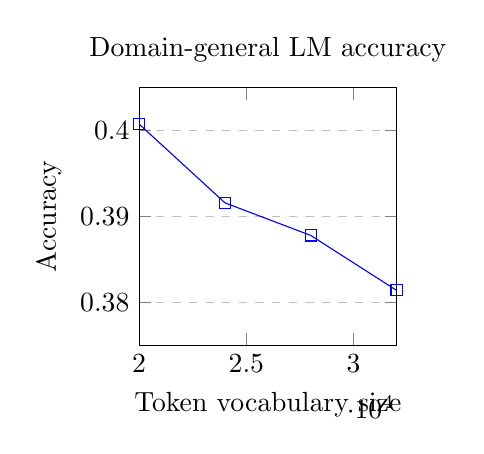
\begin{tikzpicture}
        \begin{axis}[
        title={Domain-general LM accuracy},
        width=0.4\textwidth,
        height=0.4\textwidth,
        xlabel={Token vocabulary size},
        ylabel={Accuracy},
        xmin=20000,xmax=32000,
        ymin=0.375,ymax=0.405,
        ymajorgrids=true,grid style=dashed
        ]
        \addplot[color=blue, mark=square]
        coordinates {
        (20000, 0.400775) (24000, 0.3916) (28000, 0.3878) (32000, 0.3814)
        };
        \legend{}
        \end{axis}
    \end{tikzpicture}
    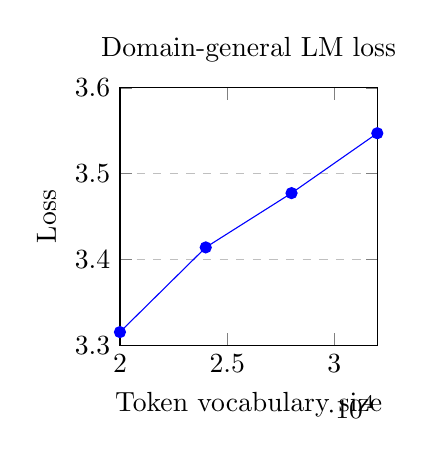
\begin{tikzpicture}
        \begin{axis}[
        title={Domain-general LM loss},
        width=0.4\textwidth,
        height=0.4\textwidth,
        xlabel={Token vocabulary size},
        ylabel={Loss},
        xmin=20000,xmax=32000,
        ymin=3.3,ymax=3.6,
        ymajorgrids=true,grid style=dashed
        ]
        \addplot[color=blue, mark=*]
        coordinates {
        (20000, 3.315355) (24000, 3.414048) (28000, 3.477319) (32000, 3.547134)
        };
        \legend{}
        \end{axis}
    \end{tikzpicture}
    \caption{A general language model accuracy (on the left) and loss (on the right) measured on a validation  set in relation to the size of the token vocabulary.}

\label{vocab:glmplot}
\end{figure}

\subsection{Accuracy of domain-specific language models}
\label{vocab:domain-specific-results}

Similarly to domain-general language models, we measure an impact of vocabulary size used on the domain-specific language model by fine-tuning four previously produced language models.

The fine-tuning begins with a training of a final layer of the model for 2 epochs. After that, an entire language model is unfrozen, and additional fine-tuning is performed for 8 more epochs. For the entire fine-tuning process, \lstinline{max_lr} is set according to table \ref{vocab:generallmlr}. The results are shown in a figure \ref{vocab:lmlrplot}.

\begin{figure}
\centering
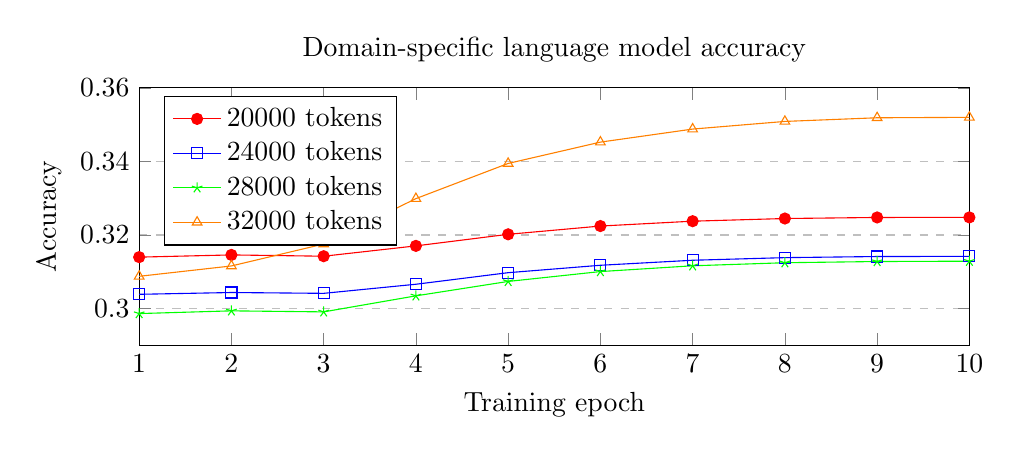
\begin{tikzpicture}[scale=1.0]
\begin{axis}[
title={Domain-specific language model accuracy},
width=\textwidth,
height=0.4\textwidth,
xlabel={Training epoch},
ylabel={Accuracy},
xmin=1,xmax=10,
ymin=0.29,ymax=0.36,
legend pos=north west,
ymajorgrids=true,grid style=dashed
]

\addplot[color=red,mark=*]
coordinates {
(1, 0.313967)
(2, 0.314566)
(3, 0.314215)
(4, 0.317025)
(5, 0.320171)
(6, 0.322419)
(7, 0.323743)
(8, 0.324468)
(9, 0.324757)
(10, 0.324771)
};

\addplot[color=blue, mark=square]
coordinates {
(1, 0.303855)
(2, 0.304343)
(3, 0.304118)
(4, 0.306591)
(5, 0.309736)
(6, 0.311752)
(7, 0.313117)
(8, 0.313828)
(9, 0.314131)
(10, 0.314177)
};

\addplot[color=green, mark=star]
coordinates {
(1, 0.298614)
(2, 0.299355)
(3, 0.299075)
(4, 0.303435)
(5, 0.307356)
(6, 0.310040)
(7, 0.311611)
(8, 0.312443)
(9, 0.312773)
(10, 0.312862)
};

\addplot[color=orange, mark=triangle]
coordinates {
(1, 0.308751)
(2, 0.311568)
(3, 0.317528)
(4, 0.329882)
(5, 0.339448)
(6, 0.345247)
(7, 0.348795)
(8, 0.350876)
(9, 0.351870)
(10, 0.351985)
};

\legend{20000 tokens, 24000 tokens, 28000 tokens, 32000 tokens}
\end{axis}
\end{tikzpicture}
\caption{A plot of domain-specific language model accuracy on a validation set depending on the size of the token vocabulary.}
\label{vocab:lmlrplot}
\end{figure}

Most notably, the accuracy of fine-tuned language models on a validation sets first decreases when a size of the token vocabulary increases, only to increase again when a vocabulary of size 32000 is chosen. 

While the language models trained on a vocabulary of size 20000 and 24000 share the exact same \lstinline{max_lr} rate and other hyperparameters, the performance of a 24000-token vocabulary language model is significantly lower than that of a 20000-token vocab one. The 32000-token vocab LM performs substantially better among the others, and the 28000-vocab LM - the worst.

\subsection{Accuracy of target classifiers}
\label{vocab:target-classifiers-results}

Finally, a relation between an accuracy of target classifiers and the token vocabulary size is measured. Target classifiers are gradually unfreezed and trained starting from the final, linear decoding layers. A constant \lstinline{lr} value of $2\cdot10^{-2}$ is used during this process.

For each model, the training process differs only in the training performed on an entirely unfrozen classifier model. Training steps utilising gradual unfreezing are shown in table \ref{vocab:class}, and the final classifier fine-tuning, performed to maximise the models' accuracy while avoiding an occurrence of overfitting, is shown in table \ref{vocab:class}.

We first compare the models' accuracy (plot \ref{vocab:classplot}) on a validation set, as well as loss on both training and a validation sets (plot \ref{vocab:classplot-loss}) in relation to the number of training epochs performed. The results indicate that a model using the largest token vocabulary $V^*$ available consistently outperforms all of the other models operating on smaller $|V^*|$. For this model, a comparison of training and validation loss shown on plot \ref{vocab:classplot-loss} leads to a conclusion that this model is not overfitting on a validation set. What's more, each model reduces its initial loss on both sets of data in the final training epoch, achieving similiar, high accuracy of over 90\% on a validation set.

\begin{table}[!t]
\centering

\begin{tabular}{ cccc }
\toprule
\multicolumn{4}{c}{Target classifier training process} \\ \midrule
Step & Epochs & Frozen to layer & Maximum learning rate \\ \midrule
1 & 2 & -1 & $lr$ \\
2 & 2 & -1 & $lr$ \\
3 & 2 & -2 & $\mathrm{slice}(lr/(2.6^4), lr)$ \\
4 & 2 & -3 & $\mathrm{slice}(lr/2/(2.6^4), lr/2)$ \\
\bottomrule
\end{tabular}
\quad
\centering
\begin{tabular}{ ccc }
\toprule
\multicolumn{3}{c}{Unfrozen classifier training process} \\ \midrule
$|V^*|$ & Epochs & Steps \\ \midrule
20000 & 1 & 2 \\
24000 & 2 & 1 \\
28000 & 1 & 1 \\
32000 & 2 & 1 \\
\bottomrule
\end{tabular}

\caption{A target classifier training process, which is performed in order to test the impact of token vocabulary size on the accuracy of the model. As a final step, final fine-tuning of a target classifier is performed depending on $|V^*|$ as shown in a rightmost table, with a \lstinline{max_lr} value of \lstinline{slice(lr/10/(2.6^4), lr/10)}.}
\label{vocab:class}
\end{table}

A comparison of models' performance is also done using a test set of labelled text document examples on trained target classifiers. A plot of relation between model's accuracy and loss on a test set \ref{vocab:results-test-set-plot} indicates that a larger amount of tokens in $V^*$ results in an increase of models' accuracy, with a 28000-token vocabulary-based model performing worse than expected.

\begin{figure}[p]
\centering
    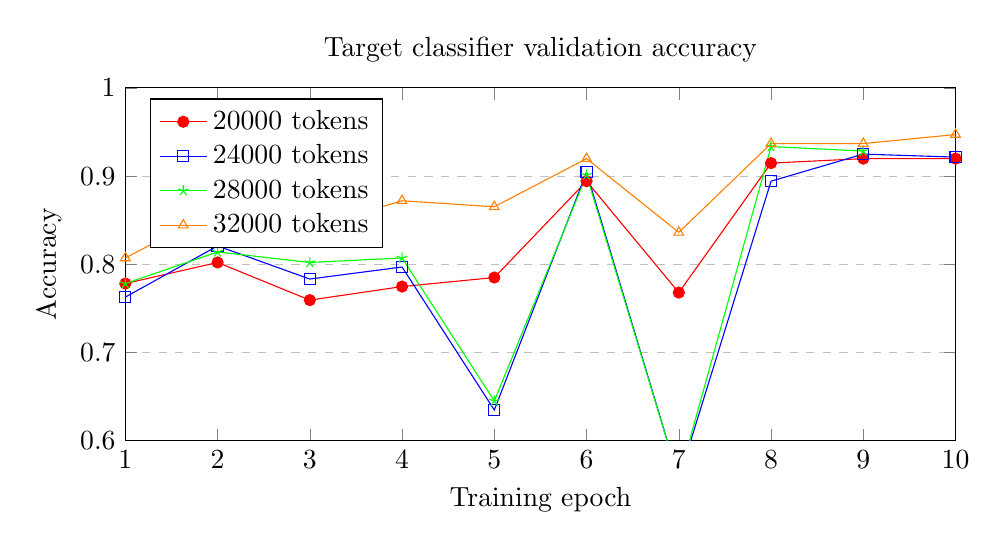
\begin{tikzpicture}[scale=1.0]
    \begin{axis}[
    title={Target classifier validation accuracy},
    width=\textwidth,
    height=0.5\textwidth,
    xlabel={Training epoch},
    ylabel={Accuracy},
    xmin=1,xmax=10,
    ymin=0.6,ymax=1,
    legend pos=north west,
    ymajorgrids=true,grid style=dashed
    ]
    
    \addplot[color=red,mark=*]
    coordinates {
    (1, 0.778157)
    (2, 0.802048)
    (3, 0.759386)
    (4, 0.774744)
    (5, 0.784983)
    (6, 0.894198)
    (7, 0.767918)
    (8, 0.914676)
    (9, 0.919795)
    (10, 0.919795)
    };
    
    \addplot[color=blue, mark=square]
    coordinates {
    (1, 0.762799)
    (2, 0.820819)
    (3, 0.783276)
    (4, 0.796928)
    (5, 0.634812)
    (6, 0.904437)
    (7, 0.556314)
    (8, 0.894198)
    (9, 0.924915)
    (10, 0.921502)
    };
    
    \addplot[color=green, mark=star]
    coordinates {
    (1, 0.778157)
    (2, 0.813993)
    (3, 0.802048)
    (4, 0.807167)
    (5, 0.645051)
    (6, 0.901024)
    (7, 0.556314)
    (8, 0.933447)
    (9, 0.928328)
    };
    
    \addplot[color=orange, mark=triangle]
    coordinates {
    (1, 0.807167)
    (2, 0.861775)
    (3, 0.841297)
    (4, 0.872014)
    (5, 0.865188)
    (6, 0.919795)
    (7, 0.836177)
    (8, 0.936860)
    (9, 0.936860)
    (10, 0.947099)
    };
    
    \legend{20000 tokens, 24000 tokens, 28000 tokens, 32000 tokens}
    \end{axis}
    \end{tikzpicture}
    \caption{A plot of target classifiers' accuracy on a validation set depending on the size of the token vocabulary. The 32000-token vocab classifier produces the highest validation accuracy in each training epoch. In epoch 7, the 28000-token vocab classifier performance drops to 0.539249 accuracy. }
    \label{vocab:classplot}
\end{figure}

\begin{figure}[p]
\centering
    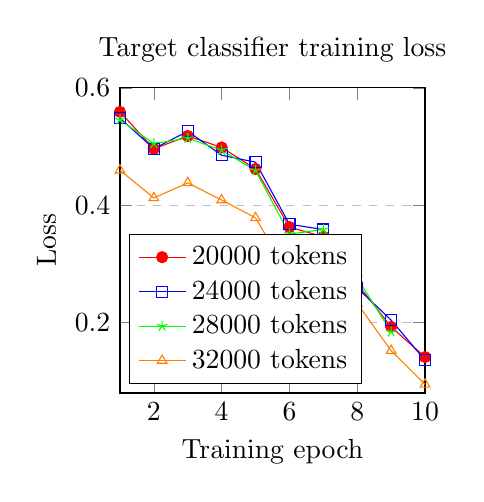
\begin{tikzpicture}[scale=1.0]
    \begin{axis}[
    title={Target classifier training loss},
    width=0.45\textwidth,
    height=0.45\textwidth,
    xlabel={Training epoch},
    ylabel={Loss},
    xmin=1,xmax=10,
    ymin=0.08,ymax=0.6,
    legend pos=south west,
    ymajorgrids=true,grid style=dashed
    ]
    
    \addplot[color=red,mark=*]
    coordinates {
    (1, 0.559043)
    (2, 0.496103)
    (3, 0.518029)
    (4, 0.498456)
    (5, 0.461751)
    (6, 0.362708)
    (7, 0.346241)
    (8, 0.265909)
    (9, 0.192528)
    (10, 0.141217)
    };
    
    \addplot[color=blue, mark=square]
    coordinates {
    (1, 0.548407)
    (2, 0.496338)
    (3, 0.525996)
    (4, 0.485223)
    (5, 0.473284)
    (6, 0.367553)
    (7, 0.358528)
    (8, 0.259165)
    (9, 0.204135)
    (10, 0.135755)
    };
    
    \addplot[color=green, mark=star]
    coordinates {
    (1, 0.545561)
    (2, 0.504994)
    (3, 0.514256)
    (4, 0.493739)
    (5, 0.459062)
    (6, 0.350794)
    (7, 0.358558)
    (8, 0.275647)
    (9, 0.184219)
    };
    
    \addplot[color=orange, mark=triangle]
    coordinates {
    (1, 0.459598)
    (2, 0.412443)
    (3, 0.438027)
    (4, 0.408843)
    (5, 0.378470)
    (6, 0.279809)
    (7, 0.320938)
    (8, 0.232594)
    (9, 0.152108)
    (10, 0.094780)
    };
    
    \legend{20000 tokens, 24000 tokens, 28000 tokens, 32000 tokens}
    \end{axis}
    \end{tikzpicture}
    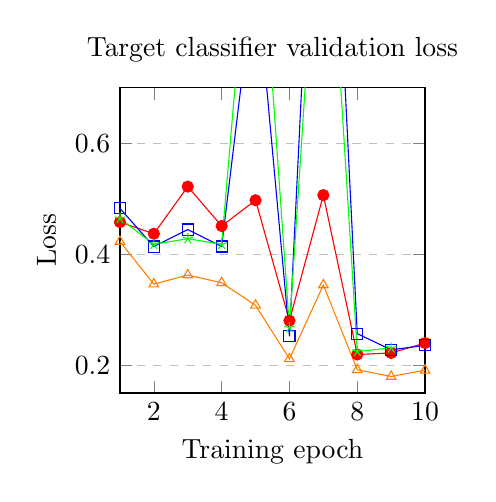
\begin{tikzpicture}[scale=1.0]
    \begin{axis}[
    title={Target classifier validation loss},
    width=0.45\textwidth,
    height=0.45\textwidth,
    xlabel={Training epoch},
    ylabel={Loss},
    xmin=1,xmax=10,
    ymin=0.15,ymax=0.7,
    legend pos=north west,
    ymajorgrids=true,grid style=dashed
    ]
    
    \addplot[color=red,mark=*]
    coordinates {
    (1,0.458031)
    (2,0.437021)
    (3,0.521998)
    (4,0.451033)
    (5,0.497400)
    (6,0.280378)
    (7,0.506661)
    (8,0.219329)
    (9,0.222112)
    (10,0.240004)
    };
    
    \addplot[color=blue, mark=square]
    coordinates {
    (1,0.482702)
    (2,0.413890)
    (3,0.444600)
    (4,0.414058)
    (5,0.920163)
    (6,0.252203)
    (7,1.497791)
    (8,0.256929)
    (9,0.227765)
    (10,0.235745)
    };
    
    \addplot[color=green, mark=star]
    coordinates {
    (1,0.464451)
    (2,0.417929)
    (3,0.428159)
    (4,0.417810)
    (5,1.138112)
    (6,0.267668)
    (7,1.203454)
    (8,0.224821)
    (9, 0.231140)
    };
    
    \addplot[color=orange, mark=triangle]
    coordinates {
    (1,0.423072)
    (2,0.346176)
    (3,0.362617)
    (4,0.348611)
    (5,0.308016)
    (6,0.211430)
    (7,0.344616)
    (8,0.191899)
    (9,0.179694)
    (10,0.190992)
    };
    
    \legend{}
    \end{axis}
    \end{tikzpicture}
\caption{A comparison of classifiers' loss on a training and a validation set. The 24000-token vocab classifier loss peaks at 1.497791 on a validation set, and the 28000-token vocab classifier - at 1.203454.}
\label{vocab:classplot-loss}
\end{figure}

\begin{figure}
\centering
    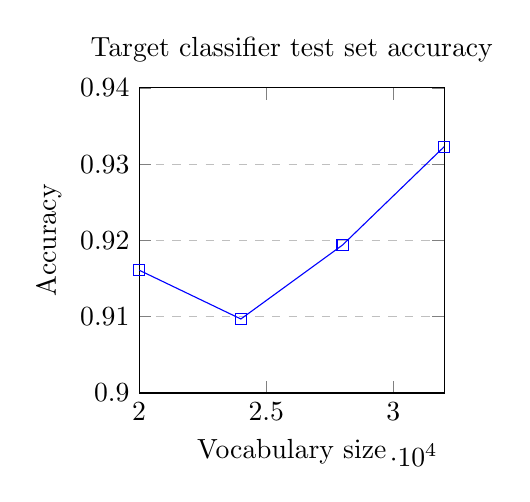
\begin{tikzpicture}[scale=1.0]
    \begin{axis}[
    title={Target classifier test set accuracy},
    width=0.45\textwidth,
    height=0.45\textwidth,
    xlabel={Vocabulary size},
    ylabel={Accuracy},
    xmin=20000,xmax=32000,
    ymin=0.90,ymax=0.94,
    legend pos=south west,
    ymajorgrids=true,grid style=dashed
    ]
    
    \addplot[color=blue, mark=square]
    coordinates {
    % (20000, 0.9290)
    % (24000, 0.9387)
    % (28000, 0.9355)
    % (32000, 0.9645)
    (20000, 0.9161)
    (24000, 0.9097)
    (28000, 0.9194)
    (32000, 0.9323)
    };
    
    \legend{}
    \end{axis}
    \end{tikzpicture}
    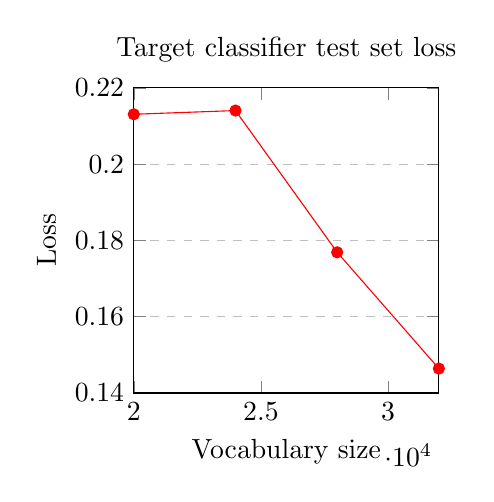
\begin{tikzpicture}[scale=1.0]
    \begin{axis}[
    title={Target classifier test set loss},
    width=0.45\textwidth,
    height=0.45\textwidth,
    xlabel={Vocabulary size},
    ylabel={Loss},
    xmin=20000,xmax=32000,
    ymin=0.14,ymax=0.22,
    legend pos=north west,
    ymajorgrids=true,grid style=dashed
    ]
    
    \addplot[color=red,mark=*]
    coordinates {
    % (20000, 0.15617181)
    % (24000, 0.13512763)
    % (28000, 0.15880364)
    % (32000, 0.10986376)
    (20000, 0.21308045)
    (24000, 0.21405071)
    (28000, 0.17687951)
    (32000, 0.14639519)
    };
    
    \legend{}
    \end{axis}
    \end{tikzpicture}
\caption{A comparison of target classifiers' accuracy (on the left) and loss (on the right) measured on a test set in relation to the size of the token vocabulary.}
\label{vocab:results-test-set-plot}
\end{figure}

\subsection{Conclusions and remarks}

While a comparison of domain-general language models' accuracy and loss (section \ref{vocab:domain-general-results}) finds that an increase of $|V^*|$ might not be beneficial, the test results performed on domain-specific language models (section \ref{vocab:domain-specific-results}) and target classifiers (section \ref{vocab:target-classifiers-results}) prove otherwise. 

This leads to a conclusion that a larger token vocabulary leads to a better performance of language models and classifiers operating on domain-specific data, which is often more nuanced than general, encyclopedic information a domain-general language model is trained on. 

However, a too high a value of $|V^*|$  may lead to a high perplexity of language models, thus decreasing the overall performance, as indicated by previous research \cite{czaplakardas:ulmfit}. For this reason, and due to the computational difficulty of pre-training a domain-general language model, an impact of $|V^*|$ was measured only in a reasonable range of tokens.

Worse than expected performance of a 24000-token vocabulary-based domain-specific language model, as well as the 24000-token vocab target classifier (section \ref{vocab:domain-specific-results}) indicates an importance of careful fine-tuning of models' hyperparameters. 

\section{Labelled data amount and target classifier performance}

In order to measure how an increase of available labelled data affects the target classifier's performance, we train several classifiers using subsets $L_i$ of examples from \lstinline{Filmweb+} labelled dataset. For each model, a subset of size $|L_i| \in \{500, 1000, 1500, 2000, 2500\}$ is chosen and used during training. Each subset $L_{i+1}$ extends contents of $L_i$ with additional 500 labelled examples from entire dataset, that is $L_1 \subseteq L_2, L_2 \subseteq L_3,\dots, L_4 \subseteq L_5$. Furthermore, each subset contains equal amount of positive and negative examples.

\subsection{Target classifiers training}

The classifiers are gradually unfrozen and trained as described in a table \ref{vocab:class}. The final-tuning training step performed on an entirely unfrozen model is identical for each of the tested models, and consists of a single, one-epoch training step with a \lstinline{max_lr} set to \lstinline{slice(lr/10/(2.6^4), lr/10)}, with an exception of the $|L_i| \in \{2000, 2500\}$, trained for two epochs in a single, final training step.

\subsection{Results and conclusions}

The performance of trained target classifiers' is measured on a test set, and the model's loss and accuracy depending on the size of a labelled dataset used for training is shown on plot \ref{dataamount:resultsplot}.

An increase of an amount of labelled training examples used for training directly impacts the accuracy of a target classifier, which increases with an corresponding increase of the dataset size. The accuracy curve shown on plot \ref{dataamount:resultsplot} indicates that an increase of labelled datasets' size has the largest effect when small datasets ($|L_i| \in \{500, 1000\}$) are used, and its impact gradually diminishes as the larger $|L_i|$ is available.

The loss of a classifier on a test set gradually increases the more labelled training examples there are available, with an exception of first two steps, where for $|L_i| \in \{500, 1000\}$ models' overfitting to a training set is observed. The more labelled training examples are available, the better resulting models' generalise.

Notably, having just 2000 labelled training examples available, the resulting classifier is able to produce over 90\% of accuracy on a test set.

In conclusion, an increase of an amount of labelled dataset's size has a positive impact on the performance of a target classifier, especially, when a limited amount is available to begin with.

\begin{figure}
\centering
    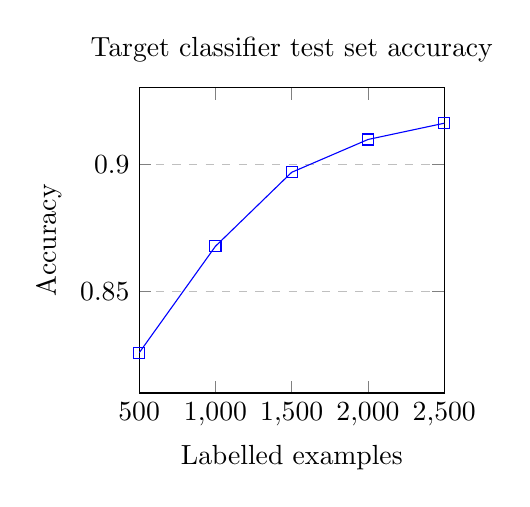
\begin{tikzpicture}[scale=1.0]
    \begin{axis}[
    title={Target classifier test set accuracy},
    width=0.45\textwidth,
    height=0.45\textwidth,
    xlabel={Labelled examples},
    ylabel={Accuracy},
    xmin=500,xmax=2500,
    ymin=0.81,ymax=0.93,
    legend pos=south west,
    ymajorgrids=true,grid style=dashed
    ]
    
    \addplot[color=blue, mark=square]
    coordinates {
    (500, 0.8258)
    (1000, 0.8677)
    (1500, 0.8968)
    (2000, 0.9097)
    (2500, 0.9161)
    };
    
    \legend{}
    \end{axis}
    \end{tikzpicture}
    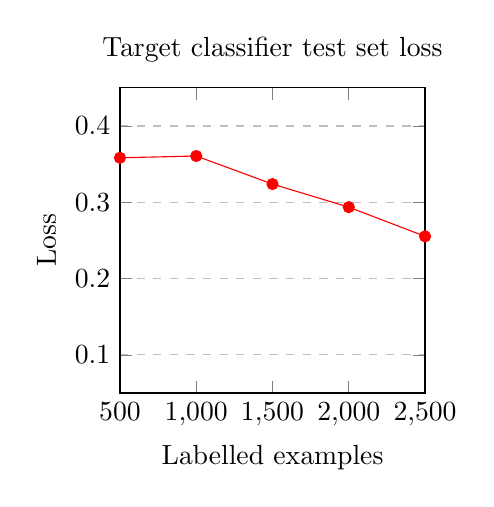
\begin{tikzpicture}[scale=1.0]
    \begin{axis}[
    title={Target classifier test set loss},
    width=0.45\textwidth,
    height=0.45\textwidth,
    xlabel={Labelled examples},
    ylabel={Loss},
    xmin=500,xmax=2500,
    ymin=0.05,ymax=0.45,
    legend pos=north west,
    ymajorgrids=true,grid style=dashed
    ]
    
    \addplot[color=red,mark=*]
    coordinates {
    (500, 0.35833675)
    (1000, 0.3606787)
    (1500, 0.32387945)
    (2000, 0.29363585)
    (2500, 0.25532904)
    };
    
    \legend{}
    \end{axis}
    \end{tikzpicture}
\caption{A comparison of target classifiers' accuracy (on the left) and loss (on the right) measured on a test set in relation to the size of the labelled dataset available.}
\label{dataamount:resultsplot}
\end{figure}

\section{Model training time}

In order to determine the amount of time needed to produce a target classifier, we perform measurements of single epoch training time of domain-general language models, domain-specific language models, and target classifiers defined in section \ref{impact:tokenvocab} for a token vocabulary of size $|V^*| \in \{24000, 28000\}$ .

Measurements are performed on a \lstinline{Vast.ai} instance equipped with a single \lstinline{GeForce RTX 2080 Ti} graphics card (see \ref{tests:env}), \lstinline{WS X299 SAGE} motherboard, \lstinline{Intel Core i7-9800X} processor and \lstinline{Samsung} SSD drive with available disk bandwith of \lstinline{546 MB/s}, producing \lstinline{18.3} teraflops of GPU performance, and rated \lstinline{19.1} according to \lstinline{Vast.ai}'s deep learning performance score, \lstinline{DLPerf}.

Models using different $V^*$ are compared in order to determine an impact of $|V^*|$ on training time.

\subsection{Results and conclusions}

The target classifier using a token vocabulary $V^*_1$ of 28000 tokens is obtained in just 4 minutes and 28 seconds more as compared to a model with $|V^*_2| = 24000$. Domain-specific language model using $V^*_1$ is obtained in 3 hours and 37 seconds more than a $V^*_2$ model, and, for the same $V^*_2$, target classifier is obtained 1 minute and 18 seconds faster than one for a smaller $V^*_1$. However, excluding the additional training step for smaller $V^*_1$, the difference amounts to just 22 seconds.

\begin{table}[ht]
\centering
\begin{tabular}{ lccc }
\toprule
\multicolumn{4}{c}{Training time measurements} \\ \midrule
\multirow{2}{*}{Model}                           & \multirow{2}{*}{Epoch} & \multicolumn{2}{c}{$|V^*|$} \\
                                                 &                        & 24000            & 28000            \\ \midrule
\multirow{10}{*}{Domain-general language model}  & 1                      & 45:08            & 45:34            \\
                                                 & 2                      & 45:05            & 45:18            \\
                                                 & 3                      & 45:05            & 45:18            \\
                                                 & 4                      & 44:48            & 45:18            \\
                                                 & 5                      & 44:53            & 45:16            \\
                                                 & 6                      & 44:49            & 45:04            \\
                                                 & 7                      & 44:51            & 45:07            \\
                                                 & 8                      & 45:02            & 45:19            \\
                                                 & 9                      & 45:01            & 45:17            \\
                                                 & 10                     & 45:03            & 44:53            \\ \midrule
& & 7:29:45 & 7:32:24\\ \midrule
\multirow{10}{*}{Domain-specific language model} & 1                      & 08:21            & 08:48            \\
                                                 & 2                      & 08:32            & 09:03            \\
                                                 & 3                      & 10:25            & 10:42            \\
                                                 & 4                      & 10:26            & 10:46            \\
                                                 & 5                      & 10:26            & 10:44            \\
                                                 & 6                      & 10:22            & 10:44            \\
                                                 & 7                      & 10:23            & 10:43            \\
                                                 & 8                      & 10:25            & 10:45            \\
                                                 & 9                      & 10:24            & 10:43            \\
                                                 & 10                     & 10:25            & 10:44            \\ \midrule
& & 1:40:20 & 1:43:57\\ \midrule
\multirow{10}{*}{Target classifier}              & 1                      & 00:31            & 00:26            \\
                                                 & 2                      & 00:31            & 00:27            \\
                                                 & 3                      & 00:33            & 00:28            \\
                                                 & 4                      & 00:32            & 00:28            \\
                                                 & 5                      & 00:38            & 00:32            \\
                                                 & 6                      & 00:41            & 00:34            \\
                                                 & 7                      & 00:52            & 00:44            \\
                                                 & 8                      & 00:49            & 00:43            \\
                                                 & 9                      & 00:54            & 00:51            \\
                                                 & 10                     & 00:56            & -\\ \midrule
& & 0:06:57 & 0:05:13 \\ \toprule
\multicolumn{2}{l}{Total training time} & 9:16:51 & 9:21:19 \\
\bottomrule
\end{tabular}
\caption{Total training time of domain-general language models, domain-specific language models and target classifiers with $|V^*| \in \{24000, 28000\}$ per training epoch.}
\end{table}

In conclusion, the target classifier can be obtained in less than 10 hours when using widely available, consumer-grade hardware. An use of more powerful graphic cards, such as \lstinline{Nvidia Tesla V100}, or multiple graphic cards for computations may result in a further decrease of total training time. 

An impact of an increase of $|V^*|$ by 4000 tokens on the training time is negligible, amounting to just 4 minutes and 28 seconds in over 9-hours-long process. However, larger token vocabularies (such as $|V^*| = 50000$) might have a more significant impact on the overall training process duration.

\section{Training epochs, iterations and target classifier performance}

We determine a significance of an amount of epochs chosen during the target classifiers' training for their validation and test set performance by training three separate models with 2, 4 and 8 epochs in each separate training instance (see test assumptions \ref{tests:assumptions}). Based on the results from this test, a model producing the best overall performance is chosen for latter study.

We also measure an impact of modifying training strategies (see table \ref{vocab:class}) applied for the best performing model's first and final layers, increasing or decreasing an amount of training epochs for chosen training instances, or adding another separate training steps. 

\subsection{Results}

\subsubsection{Global training epochs amount change and classifier performance}

Models' performance measured on a validation set (plot \ref{tests:epochs-performance-validation}) and test set (plot \ref{tests:epochs-performance-test}) leads to a conclusion that training a final classifier using the one-cycle policy with two epochs of iteration on the entire training set contents results in a model with the best overall performance. 

While an increase of training epochs amount leads to a higher validation accuracy when 4 training epochs are performed, it also results in a model overfitting to a training set, which negatively impacts it's generalisation ability. Furthermore, a further increase to 8 training epochs results in an increase of model's loss on a validation set. 

Based on these findings, the model trained with 2 epochs per training step is determined to be the best performing.

\subsubsection{Modification of training strategy for final model layer and an entirely unfrozen model}

Having determined the best performing model's training strategy we measure an impact of additional tweaks on the overall classification performance.

An increase from 2 to 8 of epochs in the first training step for the best performing model results in a slight increase of its validation set accuracy (from 0.9164 to 0.9198), with a decrease of the test set loss (from 0.2539087 to 0.22110389) and unchanged test accuracy of 0.9226.

A further decrease of epochs for the final training step from 2 to 1 leads to a decrease of validation accuracy (to 0.9061) and test loss (to 0.20510076) and an increase of test accuracy (to 0.9258) and validation loss (0.24217011). 

A final addition of 1-epoch training step with unchanged learning rate or other hyperparameters, as compared to the previous final step (see table \ref{vocab:class}) results in an additional test accuracy, test loss and validation loss increase (to 0.9323, 0.22691214 and 0.28758347 respectively) and a validation accuracy decrease (to 0.9044). 

These trials lead to an observation that an increase of training amount performed on the final layer of the model alone has a negligible impact on the model performance and, taking into account additional computational costs, can not be performed. A change in the strategy performed on an entirely unfrozen model, on the other hand, leads to a more significant difference in the model's performance.

For this reason, another modification to the training strategy (see table \ref{vocab:class}) is tested:

\begin{enumerate}
    \item A decrease of training instances performed on the final model layer from 2 to 1,
    \item A decrease of epochs in a final step from 2 to 1,
    \item An addition of final, one-epoch training step, without a change of learning rate or other hyperparameters as compared to the previously final step.
\end{enumerate}

This change results in an unchanged validation set accuracy (0.9164), but a noticeably smaller validation set loss (change from 0.2539087 to 0.23734723), higher test set accuracy (change from 0.9226 to 0.9419) and lower test set loss (change from 0.20687753 to 0.20117973). This change leads to a model achieving a better generalisation performance for new, previously unseen data, as indicated by an increase of test set accuracy.

\subsection{Conclusions}

We have found that further modifications of the training strategy described in table \ref{vocab:class} result in an increase of the overall target classifiers' performance.

While the tweaks performed on first training steps of a final classifier did not result in a significant difference, changes applied to a training policy for an entirely unfrozen model allowed for a decrease of validation and test set loss, resulting in over 94\% of model's test set accuracy, possible due to an improvement of the generalisation ability to new, unseen data.

\begin{figure}[h]
\centering
    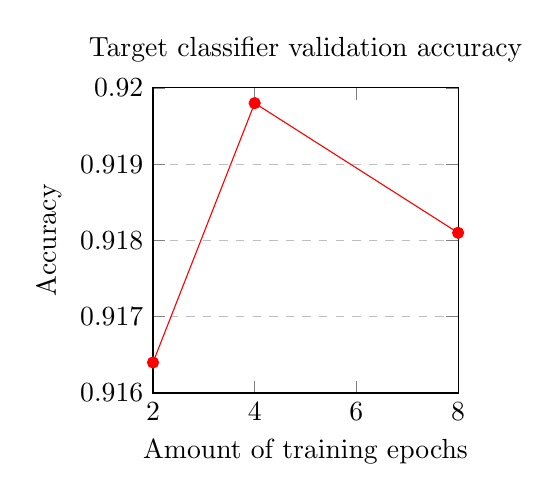
\begin{tikzpicture}[scale=1.0]
    \begin{axis}[
    title={Target classifier validation accuracy},
    width=0.45\textwidth,
    height=0.45\textwidth,
    yticklabel style={/pgf/number format/fixed,
                  /pgf/number format/precision=4},
    xlabel={Amount of training epochs},
    ylabel={Accuracy},
    ymin=0.916,ymax=0.92,
    xmin=2,xmax=8,
    legend pos=north west,
    ymajorgrids=true,grid style=dashed
    ]
    
    \addplot[color=red,mark=*]
    coordinates {
    (2, 0.9164)
    (4, 0.9198)
    (8, 0.9181)
    };
    
    \legend{}
    \end{axis}
    \end{tikzpicture}
    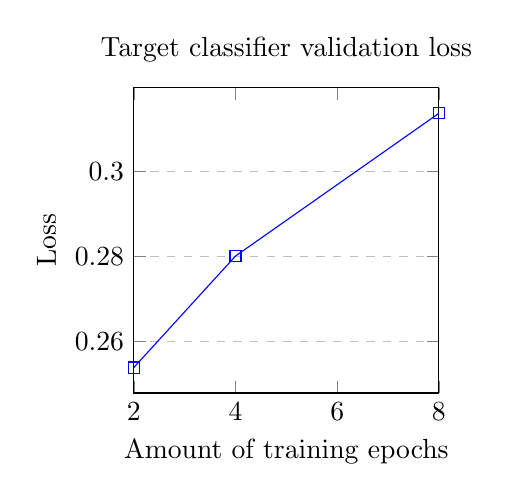
\begin{tikzpicture}[scale=1.0]
    \begin{axis}[
    title={Target classifier validation loss},
    width=0.45\textwidth,
    height=0.45\textwidth,
    xlabel={Amount of training epochs},
    ylabel={Loss},
    xmin=2,xmax=8,
    % ymin=0.2,ymax=0.32,
    legend pos=south west,
    ymajorgrids=true,grid style=dashed
    ]
    
    \addplot[color=blue, mark=square]
    coordinates {
    (2, 0.2539087)
    (4, 0.28013578)
    (8, 0.31371915)
    };
    
    \legend{}
    \end{axis}
    \end{tikzpicture}
\caption{A comparison of target classifiers' accuracy (on the left) and validation loss (on the right) in relation to the amount of epochs per single unique training instance used.}
\label{tests:epochs-performance-validation}
\end{figure}

\begin{figure}[h]
\centering
    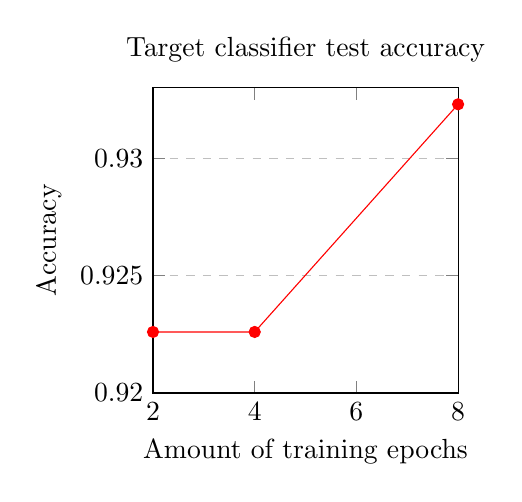
\begin{tikzpicture}[scale=1.0]
    \begin{axis}[
    title={Target classifier test accuracy},
    width=0.45\textwidth,
    height=0.45\textwidth,
    yticklabel style={/pgf/number format/fixed,
                /pgf/number format/precision=4},
    xlabel={Amount of training epochs},
    ylabel={Accuracy},
    xmin=2,xmax=8,
    ymin=0.92,ymax=0.933,
    legend pos=north west,
    ymajorgrids=true,grid style=dashed
    ]
    
    \addplot[color=red,mark=*]
    coordinates {
    (2, 0.9226)
    (4, 0.9226)
    (8, 0.9323)
    };
    
    \legend{}
    \end{axis}
    \end{tikzpicture}
    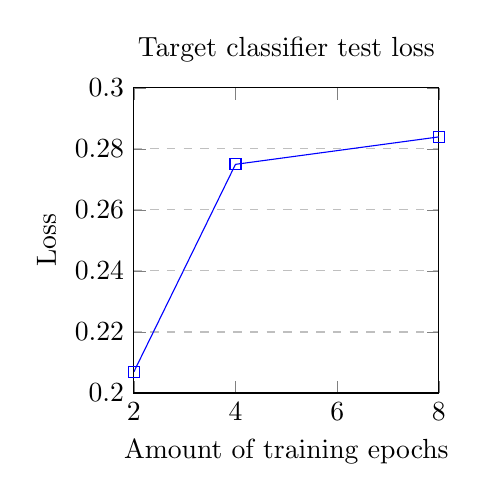
\begin{tikzpicture}[scale=1.0]
    \begin{axis}[
    title={Target classifier test loss},
    width=0.45\textwidth,
    height=0.45\textwidth,
    xlabel={Amount of training epochs},
    ylabel={Loss},
    xmin=2,xmax=8,
    ymin=0.2,ymax=0.3,
    legend pos=south west,
    ymajorgrids=true,grid style=dashed
    ]
    
    \addplot[color=blue, mark=square]
    coordinates {
    (2, 0.20687753)
    (4, 0.2749363)
    (8, 0.28393492)
    };
    
    \legend{}
    \end{axis}
    \end{tikzpicture}
\caption{A comparison of target classifiers' accuracy (on the left) and validation loss (on the right) in relation to the amount of epochs per single unique training instance used.}
\label{tests:epochs-performance-test}
\end{figure}

\chapter{Final remarks}
\label{chapter:finalremarks}

The following chapter concludes the work on a sentiment classification system, re-iterating achieved results from the work on the system, as well as key insights. It also states future directions to take in order to further explore the problem of neural networks-based document sentiment classification.

\section{Summary of work}

We have defined a problem of a document sentiment classification and provided the reader with a comprehensive background on recurrent neural network-based natural language processing, starting from important machine learning problems and ending with an perspective on impact of recent developments in the deep learning on the field of NLP.

Then, we have presented a proposed implementation of a ULMFiT-based Polish text documents sentiment classification system, based on \lstinline{plwiki} and \lstinline{Filmweb+} datasets, introducing various pre-training and fine-tuning strategies, regularisation and tokenization techniques, and manually selected hyperparameter values.

We have also provided a manual for a resulting document-level sentiment classification system, presenting an overview system's requirements, as well as usage of an available command-line interface for the purpose of performing an input document sentiment classification and training new classifier models.

Finally, in order to test an impact of different factors of an underlying machine learning model, we have performed and documented several experiments on a token vocabulary size, amount of labelled training data used and hyperparameters.

\section{Conclusions}

In conclusion, the main goal of this work, the design an implementation of a document-level sentiment classification system on a practical, real-world domain of Polish movie reviews has been successfully accomplished.

In fact, the proposed implementation achieves a test set accuracy of 94,19 \%, making it a state-of-the-art result for a real-world, long text (500 words on average) document sentiment analysis task in Polish language \cite{poleval2019,czaplakardas:ulmfit,chlasta:sentimenttwitter}, second only to performance of neural network-based implementations performing classification on short product opinions \cite{wawer:polishsentimentshorttexts,polish:sentimentsvms}.
 
\section{Future directions}

Having proven that it is possible to achieve state-of-the-art comparable performance on a Polish document-level sentiment classification task using inductive transfer learning methods on deep recurrent neural network-based classifiers produced from pre-trained and fine-tuned language models, an impact of several latest developments in the fields of NLP and deep learning on the target classification performance remains to be measured:

\begin{itemize}
\item Utilization of \emph{quasi-recurrent neural networks} as an underlying neural network infrastructure,
\item Application of \emph{subword regularization} during model training,
\item Usage of \emph{ensemble models} as a mean of improving accuracy,
\item Implementation of \emph{cross-lingual} and \emph{multi-lingual} language models \cite{howard:multifit},
\item Variable amount of unlabelled training examples used to train domain-general and domain-specific language models.
\end{itemize}

The resulting document-level sentiment classification system can be already used as a base for a commercial product used to measure the Polish audience's response towards movies or television series produced by media companies, based on reviews published on blogs and websites.

However, due to the system's modular nature being a consequence of applied inductive transfer learning approach, it can be easily applied for a problem of document-level sentiment classification in other domains of sentiment analysis, including, but not limited to political sentiment, brand sentiment, or product sentiment. This can be done for documents in a Polish language, leveraging already pre-trained domain-general language model available, by producing a model capable of working in any other language of choice.

Finally, the resulting target classifier can be applied not only for a problem of a document-level sentiment analysis, but also for any feasible text classification task of choice, such as document topic classification, spam recognition, or profanity detection. For instance, in a domain of market research, possible applications include:

\begin{itemize}
\item Detection of automatically-generated reviews by document-level binary classification (written by human, generated by software) or pattern-based classification (unusual flattery, odd formatting, etc.) used in competition research to discard unwanted opinions,
\item Verification of output from a generator of popular topics, products or articles used to fit the market demand,
\item Grouping of feedback on the product based on its features, such as price, design, or functionalities, for the purpose of future improvements.
\end{itemize}













